%!TEX root = ../dissertation.tex

\chapter{Knowledge Enhanced Neural Networks}\label{chapt:kenn}
Knowledge Enhanced Neural Networks (KENN) \cite{daniele2019kenn} is a special type of NN layer, designed for injecting logical knowledge into a pre-existing base NN. More specifically, it is a residual layer designed to be stacked after the last layer of any NN, in order to boost its predictive performances via the addition of a Prior Knowledge in the form of FOL clauses. In this chapter we will describe the theory behind KENN, its architecture, and experimental results.

\section{Theoretical Framework}\label{sec:kenn_theoretical_framework}
 We present here the theoretical framework behind KENN. The first step will be to rigorously define the symbolic language and how to link it with the theoretical framework of NNs, which consists in defining a semantic for the language. Next, we will describe the process with which the truth value of a clause can be increased, and how to integrate this method inside NNs.
 
 \subsection{Prior Knowledge and language semantic}

\begin{definition}[Prior Knowledge]
	
%	Each predicate can be applied to a specific number of constants $n$, which we will define as the \textit{arity} of the predicate.
	The Prior Knowledge is defined as a collection of formulas of a function-free first order language $\mathcal{L}$ whose signature is defined with a set of constants $\mathcal{C} = \{a_1, \dots, a_{|\mathcal{C}|}\}$ and a set of predicates $\mathcal{P} = \{p_1, \dots, p_{|\mathcal{P}|}\}$. 
	A predicate is a symbol, which can take in input a number of constants $n \geq 1$. If $n=1$, the predicate represents a property of the input constant; if $n>1$, it represents a relation between the input constants. The number $n$ is called the \textit{arity} of the predicate.
\end{definition}

\begin{definition}[Clause]
	A clause is defined to be of the following form:
	\begin{equation}
	c := \bigvee_{i=1}^k l_i, \quad l_i \neq l_j \quad \forall i \neq j.
	\end{equation}
	In this equation, $l_i$ is a literal, i.e. a formula constituted only by a $n$-ary predicate, or its negation. Specifically, when writing $l_i \neq l_j$, we mean that those two literals never share their constituting predicate. For example, the clause $A(x) \vee \neg B(x)$ is considered an acceptable clause, while $A(x) \vee B(x) \vee \neg A(x)$ is not. Also clauses have an arity, which is by definition the number of variables given in input to the clause.
\end{definition}

One example of a clause could be the following: 
\begin{equation}
c(x,y) = \neg Smoker(x) \vee \neg Friends(x,y) \vee Smoker(y),
\label{example:clause}
%TODO: può andare come correzione?
\end{equation} which, in classical logic, is equivalent to the clause $Smoker(x) \wedge Friends(x,y) \Rightarrow Smoker(y)$, but expressed as a disjunction of literals. Such a clause is constituted by two predicates: $Smoker(x)$, a unary predicate expressing the statement \say{\textit{$x$ is a smoker}}, and $Friends(x,y)$, a binary predicate which expresses the statement \say{\textit{$x$ and $y$ are friends}}. Therefore, this clause expresses the rule \say{\textit{if $x$ is a smoker and $x$ and $y$ are friends, than also $y$ is a smoker}}. Note that the variables $x$ and $y$ are supposed to be universally quantified, since our aim is to express general knowledge. We now give another definition:

\begin{definition}[Grounding of a clause]
	The grounding of an $n$-ary clause $c$, denoted as \\ $c[x_1/k_1, \dots, x_n/k_n]$,
	is the clause obtained by substituting $k_i$ to $x_i, \forall i=1,\dots,n$.
\end{definition}

Going back to the example of before, assume that $a$ and $b$ are two specific persons. Then, the grounding of clause (~\ref{example:clause}) will be $$c(x/a, y/b) = c(a,b) = \neg Smoker(a) \vee \neg Friends(a,b) \vee Smoker(b).$$

The next step is to build a semantic for the formal language $\mathcal{L}$, that is, how to interpret the symbols that we are working with. In practice, this will consist on defining a way to map constants towards a domain, and predicates to functions that go from such domain to a truth value. To clarify, consider the following example: let $a$ be a constant and let $P$ be a predicate, such that $P(x)$ expresses the statement \say{\textit{$x$ is a prime number}}. In this case, there is a natural way to define an interpretation for our symbols, that is to map constants to the domain of natural numbers and to map $P$ to the function $f: \mathbb{N}\longrightarrow\{0,1\}$, where $f(n)=1$ if $n$ is prime, and $0$ otherwise. Now, we define the semantic of $\mathcal{L}$.

\begin{definition}[Semantic of $\mathcal{L}$]
	The semantic of $\mathcal{L}$ is defined by means of a pair of functions $\left( \mathcal{I}_{\mathcal{C}}, \mathcal{I}_{\mathcal{P}} \right)$, that, together, define an \textit{interpretation} for the symbols of our language and are defined as follows:
	\begin{equation}
	\begin{aligned}[c]
			\mathcal{I}_{\mathcal{C}}: \mathcal{C} &\longrightarrow \mathbb{R}^l\\
			c&\longmapsto x,
	\end{aligned}
	\qquad \qquad
	\begin{aligned}[c]
	\mathcal{I}_{\mathcal{P}}: \mathcal{P} &\longrightarrow \left( \mathbb{R}^{nl} \rightarrow \left[0,1\right] \right)\\
	P &\longmapsto f
	\end{aligned}
	\end{equation}	
	% TODO: può andare come correzione?
	Where $n$ is the arity of the predicate $P$ and $f$ is a function that takes in input the concatenation of the interpretations of $n$ constant symbols, $\mathcal{I}_C(c_1), \dots, \mathcal{I}_C(c_n)$ and returns the truth value of $P(c_1,\dots,c_n)$. Note that, to make the notation lighter, we will omit the subscript when it's clear whether the argument of the interpretation is a literal or a constant term.
\end{definition}

With those definitions, we can already see how this theoretical framework is suitable to describe a NN. In fact, each constant symbol $c$ is mapped to a $l$-dimensional real vector, which can be seen as the feature vector characterizing the real world object identified by $c$. Another important detail is that the truth value of each literal, in our setup, is not determined by a hard assignment of $0$ or $1$, but is represented by a real number in the interval $\left[ 0,1 \right]$. 
This is a crucial point: indeed, the truth value in our semantic represents predictions of a NN, which, for classification tasks, are always expressed in terms of values in the interval $\left[0,1\right]$. The natural consequence of this choice is that, from this point on, we will have to rely on the rules of Fuzzy Logic \cite{novak1987first}, which is a generalization of the standard Boolean logic where the truth value of variables can take the value of any real number between $0$ and $1$. 

\subsection{$t$-conorm Functions}
With our definition of a semantic for $\mathcal{L}$, we can now give an interpretation for constants and predicates. The next step is to find a way to interpret clauses, or, more specifically, a way to determine the truth value of a grounded clause. We saw that, by definition, a clause is a disjunction of literals: this means that we only need a way to define the interpretation of a negated predicate and of the disjunction of two predicates. As stated above, since we are allowing truth values in the range $\left[ 0,1\right]$, we will need to use the rules of Fuzzy Logic. For computing the truth value of a negated predicate, the standard way in Fuzzy Logic is to use the Lukasiewicz Negation.

\begin{definition}[Lukasiewicz Negation]
	If $P \in \mathcal{P}$ is a predicate, then:
	\begin{equation}
	\mathcal{I}(\neg P) = 1 -\mathcal{I}(P)\footnote{Writing $1 -\mathcal{I}(P)$ is a slight abuse of notation since $\mathcal{I}(P)$ is a function. To be more precise one shoud write $\mathcal{I}(\neg P)(\mathcal{I}(c)) = 1 -\mathcal{I}(P)(\mathcal{I}(c)), \forall c$.} 
	\label{eq:lukasiewicz}
	\end{equation}
		
	
\end{definition}

So for example if the truth value of a predicate is $\mathcal{I}(P)(x) = 0.8$, the truth value of its negated copy would be $\mathcal{I}(\neg P)(x) = 0.2$. It is worth noting that this definition is equivalent to the Boolean negation when $\mathcal{I}(P) = 0$ or $\mathcal{I}(P) = 1$.

With this tool we are now able to compute the truth value of any literal. There remains to see how to define the interpretation of a disjunction of literals. To do this, we introduce the concept of $t$-conorm functions.

\begin{definition}[$t$-conorm ]
	\label{def:t-conorm}
	A $t$-conorm is a function $\perp: \left[0,1 \right]^2 \rightarrow \left[0,1 \right]$ that satisfies the following properties:
	\begin{enumerate}
		\item $\perp(a, b)=\perp(b, a)$
		\item $\perp(a, b) \leq \perp(c, d)$ if $a \leq c$ and $b \leq d$
		\item $\perp(a, \perp(b, c))=\perp(\perp(a, b), c)$
		\item $\perp(a, 0)=a$
	\end{enumerate}
\end{definition}
By definition, $\perp$ takes values in $\left[0,1 \right]^2$, but can be easily extended to $\left[0,1 \right]^n$ for any $n$, by defining:
\begin{equation*}
\perp(a_1,\dots,a_n) := \perp(a_1,\perp(a_2,\dots \perp(a_{n-1},a_n))).
\end{equation*}
In Fuzzy Logic, $t$-conorm functions are used to represent the concept of logical disjunction, and will be the tool employed to represent the interpretation of a disjunction of literals. Specifically:
\begin{equation}
\mathcal{I}(l_1 \vee \dots \vee l_n) = \perp(\mathcal{I}(l_1),\dots,\mathcal{I}(l_n)).
\end{equation}
%TODO: correzione: qui ho tolto direttamente sto pezzo...
%It is also worth specifying that $\mathcal{I}(l_1 \vee \dots \vee l_n)$ will be a function from $\mathbb{R}^{nl}$ to $\left[0,1\right]$, where $n$ is the number of literals of the clause $c := \bigvee_{i=1}^n l_i$.
With the given definitions, we have all that is needed to compute the truth value of any grounded clause. From a practical point of view, the only remaining step would be to choose a specific $t$-conorm function. KENN uses the Gödel $t$-conorm function, which is also known as the Maximum $t$-conorm and is defined as
\begin{equation*}
\perp_{max}(a,b) = \max\{a,b\},
\end{equation*}
which, as above, can be extended like follows:
\begin{equation*}
\perp_{max}(t) = \max_{i=1,\dots,l} t_i, \quad \forall t \in \mathbb{R}^l.
\end{equation*}

We are now finally ready to fully understand how this theoretical framework is able to describe the predictions of a NN. Suppose that we have a dataset $\mathcal{X}=\{x_1, \dots, x_n\}, x_i\in\mathbb{R}^l$, where each $x_i$ belongs to one or more classes $\left( P_1, \dots, P_m \right)$. The task in which the NN must learn to classify each input into one or more output classes is known  in Machine Learning as a multilabel classification problem. To tackle this kind of task, a NN architecture will present, in the last layer, $m$ output units, each of which will be finally subject to a sigmoidal activation function. After training, the NN will have learned to approximate a function $h(x_i) = y_i \in \mathbb{R}^m$, where $(y_i)_j = \mathbb{P}(x_i\text{ belongs to class }j).$ Now, if we consider:
\begin{enumerate}
	\item $\mathcal{P} = \{P_1,\dots,P_m\}$ to be predicates defined as $P_i(x) = $ \say{$x$ belongs to class $P_i$};
	\item $\{x_1,\dots, x_n\}$ to be the interpretations of the constants $\mathcal{C} = \{c_1,\dots,c_n\}$, which represent the real-world objects of our dataset,
\end{enumerate}  it is clear that the entries of $y_i$ can be seen as truth values of the predicates $\{P_1,\dots,P_m\}$. More formally:
\begin{equation}
(y_i)_j = \mathcal{I}_{NN}(P_j)(x_i), \quad \forall i=1,\dots,n, \forall j=1,\dots,m.
\end{equation}
Hence, the whole NN defines an interpretation for each predicate $P_i$, which we denoted as $\mathcal{I}_{NN}$. Therefore, given a clause $c := \bigvee_{i=1}^k l_i$ and given a collection of feature vectors $\{x_1,\dots,x_d\}$  (where $d$ is the arity of $c$), then the truth value of the grounded clause predicted by the NN will be $\perp((y_c)_1,\dots,(y_c)_k)$, where:
\begin{equation}
\label{eq:yc}
y_c \in \mathbb{R}^k, \quad(y_c)_i = \begin{cases}
\mathcal{I}_{NN}(l_i) \text{ if } l_i \text{ is not a negated predicate}\\
1-\mathcal{I}_{NN}(l_i) \text{ otherwise.}
\end{cases}
\end{equation}

The intuition behind KENN is very simple: given the vector $y$ of predictions of the NN, a new layer is added at its end with the aim to modify $y$ and obtain a new vector of predictions $y'$, of the form $y'=y+\delta$, such that $y'$ improves the truth value of each clause present in the base knowledge and, at the same time, keeps the quantity $\|y'-y\|_2$ minimal. It is worth noticing that this new layer introduced by KENN, called Knowledge Enhancer (KE), is a kind of residual layer, since it learns to represent the quantity $\delta = y'-y$.

\subsection{$t$-conorm Boost Functions}
The next problem is to understand how to improve the truth value of a single clause $c \in \mathcal{K}$. Since this truth value is represented by a $t$-conorm function, this involves finding a way to let the value of $\perp(y_c)$ rise by manipulating the value of $y_c$, where $y_c$ is the vector of truth values of the literals contained in clause $c$, defined in equation (\ref{eq:yc}). To do this, we define a new class of functions.

\begin{definition}[$t$-conorm Boost Function (TBF)]
	A function $\delta:[0,1]^{n} \rightarrow[0,1]^{n}$ is a $t$-conorm Boost Function (TBF) if:
	$$
	0 \leq t_{i}+\delta(t)_{i} \leq 1  \quad \forall n \in \mathbb{N} \quad \forall t \in[0,1]^{n}.
	$$
	Let $\Delta$ denote the set of all TBFs.
\end{definition}
From the definition follows a simple but essential result.

\begin{lemma}
	Given any $t$-conorm $\perp$ and $\delta \in \Delta$, it holds that:
	$$ \perp(t) \leq \perp(t + \delta(t)).$$
\end{lemma}
\begin{proof}
	By definition of TBF, $\delta(t)_i \geq 0$. This implies that $$t_i \leq t_i + \delta(t)_i, \quad \forall i=1,\dots,n.$$By the monotonicity of $t$-conorms (i.e. property 2 of Definition \ref{def:t-conorm})
	, it follows that $\perp(t) \leq \perp(t+\delta(t))$.
\end{proof}

The purpose of such TBF $\delta$ is to update the value of $y_c$ in such a way that the truth value of the clause, $\perp\left(y_c\right)$, increases. The problem is now how to choose such a TBF. It is clear that not all the $\delta \in \Delta$ would be useful: for example, one could choose the function $\delta(y_c)_i = 1-(y_c)_i$. In this way, we would obtain an updated truth value of $1$ for any literal, independently of $y_c$. This of course would be pointless, and would render the predictions of the base NN useless. For this reason another requirement for $y'$ is needed. Specifically, as we already mentioned, KENN is built in such a way that the learnt delta improves the $t$-conorm value in a minimal way. To be more rigorous, we will now formally define the concept of a minimal TBF.

\begin{definition}[Minimal TBF]
	A function $\delta \in \Delta$ is minimal with respect to a norm $\|\cdot\|$ and a $t$-conorm $\perp$ if and only if:
	$$
	\left\|\delta^{\prime}(t)\right\|<\|\delta(t)\| \Rightarrow \perp\left(t+\delta^{\prime}(t)\right)<\perp(t+\delta(t)), \quad \forall \delta^{\prime} \in \Delta, \quad \forall n \in \mathbb{N}, \quad \forall t \in[0,1]^{n}.
	$$
\end{definition}

As mentioned above, KENN works with the Gödel $t$-conorm function and the $L_p$ norm $\|x\|_p = \left( \sum_{i=1}^n |x_i|^p \right)^{\frac{1}{p}}$.
The next step at this point is to find such a minimal TBF. In the following result, we present a possible form that a minimal TBF can assume.
\begin{theorem}
	\label{thm:min_tbf}
	For any function $f: \mathbb{R}^{n} \rightarrow \mathbb{R}$ and for any vector $t \in \left[0,1\right]^n$, we define \mbox{$\delta^{f}: \mathbb{R}^{n} \rightarrow \mathbb{R}^{n}$} as
	$$
	\delta^{f}(t)_{i}= \begin{cases}f(t) & \text { if } i=\arg\max_{j=1}^n t_{j} \\ 0 & \text { otherwise }\end{cases}
	$$
	Let $f: \left[0,1\right]^{n} \rightarrow \left[0,1\right]$ satisfying $0 \leq f(t) \leq 1- \max_{j=1}^n t_j$. Then, $\delta^f$ is a minimal TBF for the Gödel $t$-conorm function and the $L_p$ norm.
\end{theorem}
\begin{proof}
	$\delta^f$ is a TBF. Indeed $\delta^f(t) \geq 0$ and $0 \leq t_i + \delta^f(t_i) \leq 1$ because $f(t) \leq 1- \max_j t_j$. Therefore we only need to prove that $\delta^f$ is minimal. Take $\delta \in \Delta$, with $\|\delta(t)\|_p < \|\delta^f(t)\|_p$. We have to show that $$\perp\left(t+\delta\left(t\right)\right) < \perp\left(t+\delta^f\left(t\right)\right).$$ 
	Now define $j=\arg\max_k \left(t_k + \delta(t)_k\right)$. By definition of the Gödel $t$-conorm we can immediately derive that:
	\begin{equation}
	\perp(t+\delta(t)) = t_j+\delta(t)_j.
	\label{eq:proof1}
	\end{equation}
	Now, defining $i=\arg\max_k t_k$, using the same reasoning and exploiting the definition of $\delta^f$ it follows that:
	\begin{equation}
	\perp(t+\delta^f(t)) = t_i + f(t).
	\label{eq:proof2}
	\end{equation}
	By combining (\ref{eq:proof1}) and (\ref{eq:proof2}) and noting that by definition $t_i \geq t_j$, the last step is to prove that $f(t) > \delta(t)_j$. To do this we exploit the definition of $L_p$ norm as follows:
	
	$$ \delta(t)_j = (|\delta(t)_j|^p)^\frac{1}{p} \leq \left(\sum_{k=1}^{n}|\delta(t)_k|^p \right)^{\frac{1}{p}} = \|\delta(t)\|_p < \|\delta^f(t)\|_p = f(t). $$ 
	Where the last inequality follows from the definition of $\delta^f(t)$.
	
\end{proof}
%This makes sense even from an intuitive point of view: since $\perp (a) = \max_ia_i$, the only way to increase $\perp(a)$ is to let $\max_{i} a_i$ increase, without modifying the rest of the $a_j, j \neq i$.

\subsection{Applying TBFs to preactivations} 
\label{sec:tbf_preac}
There is a problem with the definition of $\delta^f$: there is a specific constraint $f(t) \leq 1 - \max_i t_i$ that limits the number of candidates for $f$. Indeed, this is imposed to ensure that each entry of the final output $y_c'= y_c + \delta^f(y_c)$ will be in $\left[0,1\right]$. There is a natural way to solve this impracticality: since we are assuming a multilabel classification scenario, the final $m$ output units of the NN will pass through a sigmoidal activation function. More specifically, $y_i$ will be of the form:
\begin{equation*}
y_i = \sigma(z_i) = \frac{1}{1+e^{-z_i}}, \quad \forall i=1,\dots,m,
\end{equation*}
where $z$ is the vector of preactivations from the NN. For this reason, KENN exploits the fact that $\sigma$ takes only values in $\left[0,1\right]$ by applying the TBF directly on the preactivations $z$. In fact, it is clear from an intuitive point of view that one can apply any delta to the preactivations vector, and at the same time always be sure that the final output will be in $\left[0,1\right]$. In this way, the constraint on $f$ is no longer needed. 
However, recall that the input for the TBF at the activation level is $y_c$ (defined in equation (\ref{eq:yc})), which is the vector of truth values for the literals present in clause $c$. Therefore, in the same way, we will need to define $z_c$, the vector of preactivations for the literals of clause $c$. There is one problem though: we don't know how to define the preactivation of a negated literal, i.e. we don't know how to derive $z_{\neg A}$ from $z_A$. In fact, recall that in equation (\ref{eq:lukasiewicz}) we defined the interpretation of a negated predicate, where we knew that the truth values were well defined in the interval $\left[0,1\right]$. Now we are dealing with preactivations, which cannot be considered truth values in the Fuzzy Logic theoretical framework. However, this problem can be easily solved by exploiting the following property of the sigmoid activation function:
	\begin{equation*}
	1 - \sigma(x) = \sigma(-x).
	\end{equation*}
	Now it's easy to see that, since $y_{\neg A} = 1 - y_A$, we can define:
	\begin{equation*}
	z_{\neg A} = -z_A.
	\end{equation*}
	Notice that we are not introducing any new concepts: instead we are just redefining quantities that were already mentioned at the activation level, to the preactivation level.
	In this way, we can finally define $z_c := \left(z_{l_1}, \dots, z_{l_k}\right)$ for every clause $c := \bigvee_{i=1}^k l_i$ of the knowledge. We refer to the process of transforming from $z$ to $z_c$ as the \textit{selection} step.

Going back to the main problem, in the next theorem we prove formally that applying a minimal TBF on the preactivations $z_c$ is equivalent to applying a minimal TBF on $y_c$.
\begin{theorem}
	Given any function $f:\mathbb{R}^n\rightarrow\mathbb{R}$, and given $t = \sigma(v), v\in 
	\mathbb{R}^n$, the function:
	\begin{equation}
	\delta^g(t) = \sigma(v+\delta^f(v))-\sigma(v)
	\label{eq:delta_g}
	\end{equation}
	is a minimal TBF under the Gödel $t$-conorm and the $L_p$ norm.
\end{theorem}
\begin{proof}
	By definition we know that $v = \sigma^{-1} (t)$, hence we can rewrite equation (\ref{eq:delta_g}) as:
	$$ t + \delta^g(t) = \sigma(v + \delta^f(v)).$$
	From the definition of sigmoid activation function it easily follows that $0 \leq t + \delta^g(t) \leq 1$. To prove that $\delta^g$ is a TBF we have to show that $\delta^g(t) \geq 0$.
	We note a few details: $\sigma$ is monotonic increasing, which means that:
	$$
	\underset{j=1}{\operatorname{argmax}}{ }_{j=1}^{n} \sigma\left(v_{j}\right)=\underset{j=1}{\operatorname{argmax}} v_{j}.
	$$
	Another implication of the monotonicity of $\sigma$ is that:
	$$
	f(v) \geq 0 \Rightarrow \sigma\left(v_{i}+f(v)\right) \geq \sigma\left(v_{i}\right).
	$$
	This implies that $\delta^g(t)=\sigma(v+\delta^f(v)) - \sigma(v) \geq 0$.
	We now define the function $g(t) = \sigma(v_i + f(v)) - \sigma(v_i)$, where $i = \arg\max_j v_j$. It's easy to see that this $g$ is the function associated to our $\delta^g$. In fact:
	\begin{align*}
	\delta^g(t)_i &= \sigma(v + \delta^f(v))_i - \sigma(v)_i \\
	&=\begin{cases}
	g(t) &\text{if } i=\arg\max_j t_j\\
	0 &\text{otherwise.}
	\end{cases}
	\end{align*}
	Therefore, Theorem \ref{thm:min_tbf} guarantees that $\delta^g$ is a minimal TBF under the Gödel $t$-conorm and the $L_p$ norm.
\end{proof}
Note that $\delta^g(y_c)$ is not directly computed in KENN but it's indirectly induced by applying $\delta^f$ on $z_c$. 

Applying the TBF directly on the preactivations has also another remarkable advantage. Indeed, it is known that it is  possible to interpret the value of the preactivation of the $i$-th output neuron as the \say{confidence} of the NN that the current feature vector is to be classified in the $i$-th class. 
This \say{confidence} is not yet a probability, but a generic scalar value $x \in \mathbb{R}$; it will become a probability when transformed with the sigmoid activation function: $\sigma(x) \in \left[0,1\right]$. More specifically we know that:
\begin{itemize}
	\item $x \gg 0$ means high confidence of being classified in the $i$-th class. This follows from the fact that $\lim_{x\rightarrow +\infty} \sigma(x) = 1$;
	\item $x \ll 0$ means high confidence of \textit{not} being classified in the $i$-th class. This follows from the fact that $\lim_{x\rightarrow -\infty} \sigma(x) = 0$;
	\item $x \approx 0$ corresponds to a highly uncertain decision. This follows from the fact that $\sigma(x) \approx 0.5$ if $x \approx 0$.
\end{itemize}

%TODO: sicuro delle correzioni fatte ieri sera?
By observing the shape of the sigmoid activation function we can notice that when $|z| \gg 0$ (high confidence in the NN predictions), even large deltas on the preactivations produce very small changes. 
More rigorously, $\lim_{|x| \rightarrow \infty} |\sigma(x+\delta)-\sigma(x)| = 0, \forall x\in \mathbb{R}, \delta \gg 0$. On the contrary, when $x \approx 0$, even small deltas on the preactivations produce high modification at the activation level. 
This will result in the following behavior: if the NN is highly confident of its decision, then logical rules will not modify too much the result of the NN predictions. On the contrary, in the cases where the NN is uncertain of its decision, our base knowledge will intervene and give higher modifications on the final predictions. This conforms to the intuition that KENN should produce minimal changes in the original predictions. These key concepts are further illustrated in Figure \ref{fig:preacs_deltas_example}.

\begin{figure}[h!]
	\centering
	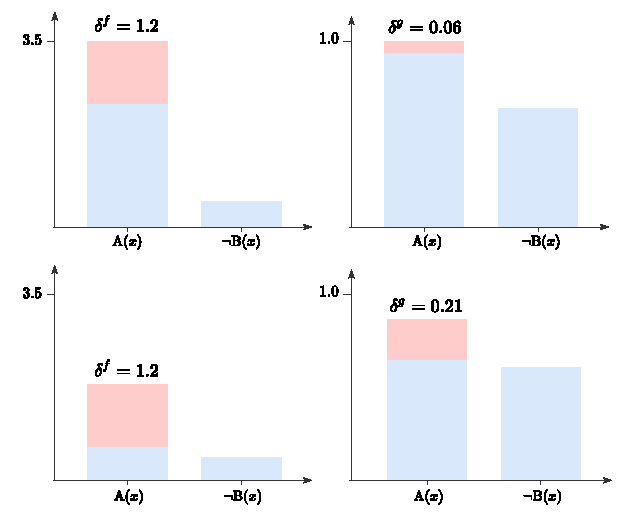
\includegraphics[width=0.75\textwidth]{figures/preac_deltas_example.pdf}
%	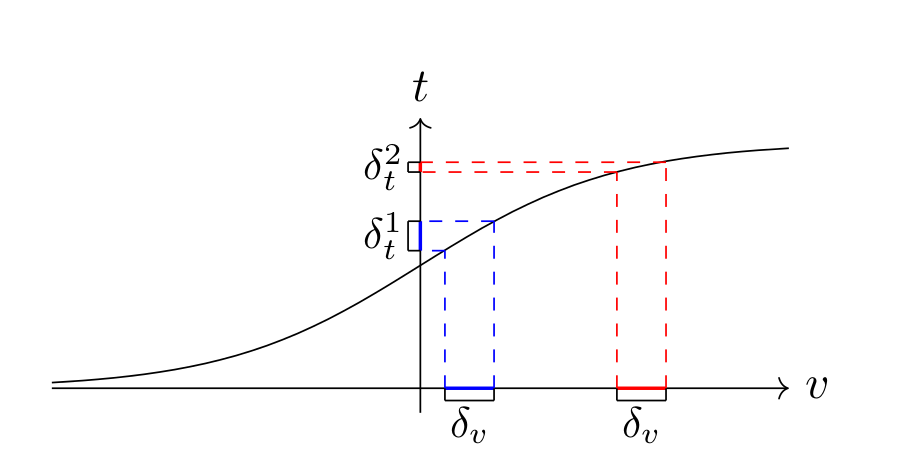
\includegraphics[width=0.7\textwidth]{figures/sigmoid_shape_example.png}
	%TODO: refine this caption!!!
	\caption{On the left, example preactivations for the clause $\operatorname{A}(x) \vee \neg \operatorname{B}(x)$ are shown. For both the examples, the same delta ($\delta^f$) is applied to these preactivations. In the first example, the NN has a high confidence, while in the second one it is much lower. We can see how, when applying the activation function, the actual delta ($\delta^g$) is much smaller in the first case and larger in the second. This is due to the shape of the sigmoid activation function itself.  }
	\label{fig:preacs_deltas_example}
\end{figure}

As we already mentioned, the minimal TBF directly modeled by KENN is the one we called $\delta^f$. From its definition, we know that the magnitude of the produced delta is determined by the definition of $f$. One of the most important features of KENN is that, by design, it learns to give the proper \textit{importance} to each clause in the base knowledge: this precise feature of the model gives also a way to find such function $f$. Specifically, for each clause $c$ a learnable parameter $w_c$ is defined so that the produced delta for $c$ is:
\begin{equation*}
	\delta^{w_c}(z_c)_i = 
	\begin{cases}
	w_c \quad &\text{if } i = \arg\max_{j=1}^n(z_c)_j \\
	0 \quad &\text{otherwise.}
	\end{cases}
	\end{equation*}
From this definition it's now clear that the function $f$ we were looking for is not actually the same for all the clauses in the base knowledge, but it is defined for each different clause and it's equal to the constant function $f_c(z_c) = w_c, \quad w_c \in \left[0, \infty\right]$. 
There is one last problem: while it's true that the function $\delta^{w_c}$ is a minimal TBF, the implementation of this kind of functions inside a NN is unfeasible since they are not differentiable. For this reason KENN uses a soft approximation of $\delta^{w_c}$, defined as:
\begin{equation}
	\delta_s^{w_c}(z_c)_i = w_c \cdot \operatorname{softmax}(z_c)_i = w_c \cdot \frac{e^{(z_c)_i}}{\sum_{j=1}^ne^{(z_c)_j}}.
	\label{eq:soft_approx_delta}
	\end{equation}
%Recall our notation: we defined with $y \in \mathbb{R}^m$ the vector of predictions from the NN. Specifically, we now define with $y_A$ the truth value relative to $A$, where $A$ is a generic grounded predicate of our language. We also define $z_A=\sigma^{-1}(y_A)$.
% Now, we note that equation (\ref{eq:soft_approx_delta}), tells us that the produced $\delta$ is always $m$-dimensional, where $m$ is the number of output classes. 
%This however is not desirable: in fact, in general, not all the clauses in our base knowledge contain all the predicates of our language. For example, given $\mathcal{P}=\{A,B,C\}$, the clause $c = A \vee \neg B$ contains only two of the three predicates in the language. Therefore, we would like this specific clause to not modify in any way $z_C$. 
There is still, however, one additional step to describe in order to fully understand how KENN produces a vector of deltas. Let $\mathcal{K}$ be the set of clauses in our knowledge, and $\{w_c\}_{c\in\mathcal{K}}$ their corresponding weights. For every clause $c\in \mathcal{K}$ we want to obtain a new delta, namely $\delta^c \in \mathbb{R}^m$, which contains one value for each predicate in the clause and is defined as follows:
\begin{equation}
\delta_{A}^{c}= \begin{cases}\delta_{s}^{w_{c}}\left(z_{c}\right)_{A} & \text { if } A \in c \\ -\delta_{s}^{w_{c}}\left(z_{c}\right)_{\neg A} & \text { if } \neg A \in c \\ 0 & \text { otherwise }\end{cases}, \quad \forall A \in c
\label{eq:delta_c}
\end{equation}
This newly defined delta, $\delta^c$, will be the change obtained from clause $c$ and will be summed to $z$ to obtain the updated prediction. More specifically:

$$y' = \sigma(z + \delta^c).$$

In Figure \ref{fig:delta_single_clause}, an example of computation of the $\delta^ c$ vector is provided.

\begin{figure}[h!]
	\centering
	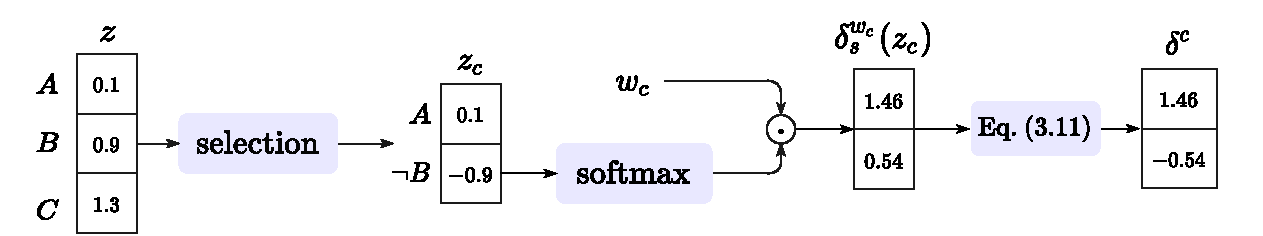
\includegraphics[width=\linewidth]{figures/delta_single_clause.pdf}
	\caption{Example with all the steps needed to compute $\delta^c$ for the clause $A \vee \neg B$ starting from the vector of preactivations $z$; for this example $w_c=2$. We refer to this process as \textit{clause enhancement}.}
	\label{fig:delta_single_clause}
\end{figure}


\subsection{Increasing the satisfaction of the Knowledge}
In the previous section we found out how KENN produces a vector of changes $\delta$ to be applied to the original NN predictions, but only considering a single clause. That would suffice in the cases where the knowledge is constituted only by a single clause, but in real applications a higher number of logical rules will be desirable. Therefore, the next and final problem is to understand how KENN takes all the deltas from all the clauses and produces a single vector of changes. This particular step of aggregation is critical, as it constitutes one of the best features of KENN, but at the same time one of its bigger inaccuracies. This is because, to aggregate the contributions from all the clauses $c \in \mathcal{K}$, KENN just sums the contributions. Specifically, the final prediction is defined as follows:
\begin{equation}
\label{eq:deltas_sum}
y'=\sigma(z + \sum_{c\in\mathcal{K}}\delta^c).
\end{equation}
This particular choice makes KENN really fast at inference and learning time, increasing scalability. At the same time, though, this makes the risk of inconsistencies higher. For example, the same predicate can appear negated in one clause, and not negated in another clause: in this way the delta for the first one will be negative while it will be positive for the second one. In this way, the two deltas may cancel out rendering the contributions of the two clauses less effective.


\section{KENN Architecture}
\label{sec:kenn_architecture}
In this section we describe the architecture of the KENN layer in details. First, we will describe the basic functioning for the case where the knowledge is constituted only by unary clauses. Then, in Section \ref{sec:relational_kenn}, we will describe how KENN is able to handle binary clauses. Note that, theoretically, KENN can be extended to work with clauses of any arity. However, for now it has been implemented to work with unary and binary clauses, which are also the most common use cases. All the contents of this section have been implemented as a Python 3 package, based on TensorFlow 2 \cite{abadi2016tensorflow} and all the source code is publicly available on Github\footnote{\url{https://github.com/DanieleAlessandro/KENN2}}.

As described above, the core functionality of KENN is the \textit{clause enhancement}, i.e. the creation of a vector $\delta$ which, summed to the vector of preactivations $z$ from a NN, produces a modified vector of predictions $y'$ which increases the truth value of the relative clause.
 The architecture that takes care of this task is the Clause Enhancer (CE): this submodule takes in input the full vector of preactivations from the original NN and computes the vector of deltas described in equation (\ref{eq:delta_c}). For each clause in the base knowledge, a CE will be instantiated. Note how the CE does not take in input a single vector of preactivations at a time, but works in parallel taking in input mini-batches of data. The details of the architecture of the CE are described in Figure \ref{fig:ce}.
\begin{figure}
	\centering
	\begin{subfigure}{.5\textwidth}
		\centering
		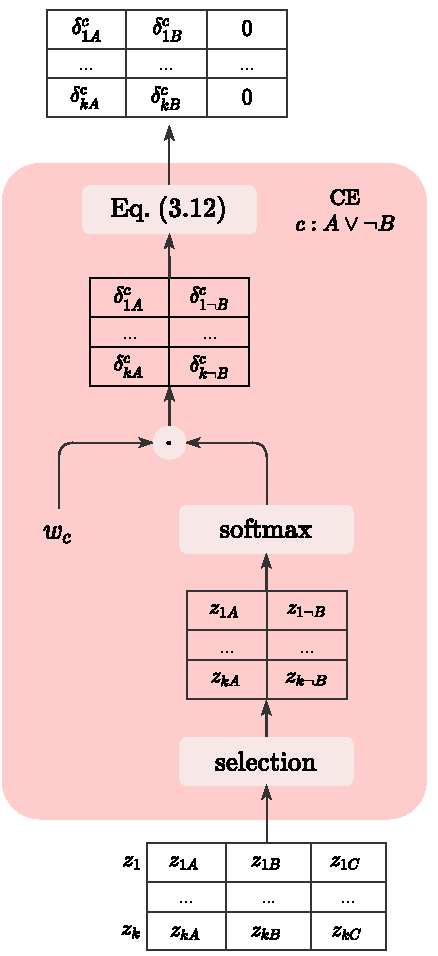
\includegraphics[width=0.8\linewidth]{figures/CE.pdf}
		\caption{The Clause Enhancer (CE) module.}
		\label{fig:ce}
	\end{subfigure}%
	\begin{subfigure}{.5\textwidth}
		\centering
		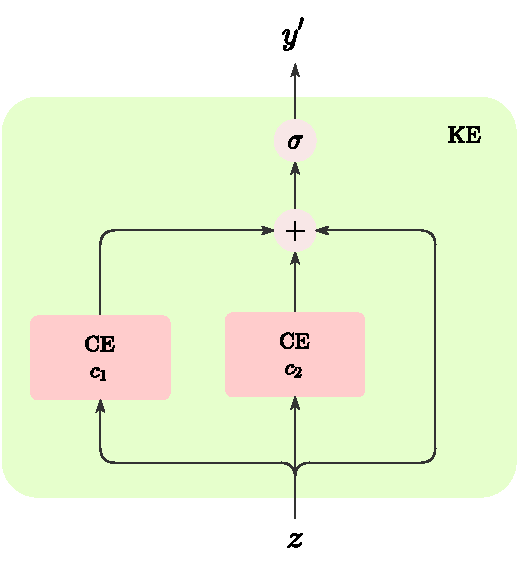
\includegraphics[width=0.9\linewidth]{figures/KE.pdf}
		\caption{The Knowledge Enhancer (KE) module.}
		\label{fig:ke}	
	\end{subfigure}
	\caption{Illustration of the KENN architecture. Images are replications of the illustrations provided in \cite{daniele2019kenn}.}
	\label{fig:kenn_architecture_unary}
\end{figure}
Specifically, the CE takes in input the mini-batch of preactivations $\{z_1,\dots,z_k\}$ coming from the base NN, and for each sample in the mini-batch performs the following operations:
\begin{enumerate}
	\item Performs the \textit{selection} step;
	\item Computes the vector of deltas according to equation (\ref{eq:soft_approx_delta});
	\item Transforms the delta vector according to equation (\ref{eq:delta_c})
\end{enumerate}
Once every CE has produced a vector of deltas, the next step is to aggregate them by summing them up. The module that performs this operation is called the Knowledge Enhancer (KE), which is shown in Figure \ref{fig:ke}. More specifically, the KE performs the following operations:
\begin{enumerate}
	\item Takes all the preactivations from the NN as inputs, and instantiates a CE for each clause in the knowledge base;
		\item Sums the produced vector of changes from all the CEs, obtaining a final delta vector;

	\item It sums the obtained delta with the original preactivations vector;
	\item Applies the sigmoid activation function.
\end{enumerate}


 These steps produce the final vector of modified predictions $y'$. Notice that the KE is the implementation of equation (\ref{eq:deltas_sum}).
 
 \section{KENN for relational data}
 \label{sec:relational_kenn}
 
As we said, KENN can also handle relational data; specifically, thanks to its general approach, KENN can theoretically handle clauses with any arity. Nevertheless, for simplicity, we will just describe how it is possible to handle the case of binary clauses. In order to integrate binary clauses, the first step is to split the base knowledge into two disjoint subsets of clauses $\mathcal{K}_U$ and $\mathcal{K}_B$, containing the unary and binary clauses respectively. In this way, the set of all the clauses constituting the Prior Knowledge is denoted as \mbox{$\mathcal{K} = \mathcal{K}_U \cup \mathcal{K}_B$}. The intuition at the base of KENN remains the same: starting from initial predictions $z$, we will need to produce a vector of deltas $\delta$. The only difference, is that $\delta$ will be the sum of two different deltas, one produced just by unary clauses and the other just by binary clauses. More in details, this consists in modifying equation (\ref{eq:deltas_sum}) as follows:
 
 \begin{equation}
 \label{eq:binary_kenn_eq}
 y'=\sigma(z + \sum_{c\in\mathcal{K}_U}\delta^c + \sum_{c\in\mathcal{K}_B}\delta^c).
 \end{equation}
Note that the procedure to compute the quantity $\sum_{c\in \mathcal{K}_U}\delta^c$ is the one we described before, since it deals just with unary clauses. The only thing left to define is how to compute a delta vector starting from a binary clause. 

\subsubsection{Table representation of binary data}

In order to deal with binary clauses, KENN represents truth values of every grounded predicate inside two different matrices: $U$ and $B$. Matrix $U$ has one row for each constant, one column for each unary predicate and an additional column containing an identifier for each object. Matrix $B$, instead, has one row for each couple of objects: specifically, for each pair of objects such that there is a binary relation between them. The first two columns of $B$ contain the identifier indices of the pair of objects, while the remaining columns contain the preactivations for each binary predicate, grounded on that pair of objects. So, in the case of $n$ unary predicates, $m$ binary predicates, $p$ total objects and $q$ couples of objects, $U$ and $B$ will have dimensions $p \times (n+1)$ and $ q \times (m+2)$ respectively. Figure \ref{fig:KENNrelationalrepr} shows an example with a visualization of $U$ and $B$. With those newly defined matrices, equation (\ref{eq:binary_kenn_eq}) can be implemented as follows:
\begin{equation*}
	\begin{cases}
	y_u' = \sigma(U+\delta U)\\
	y_b' = \sigma(B + \delta B),
	\end{cases}
	\end{equation*}
	where $y_u'$ and $y_b'$ are the final predictions for the unary and binary predicates respectively, and $\delta U$ and $\delta B$ are the delta matrices that need to be computed.
 
 \begin{figure}
 	\centering
 	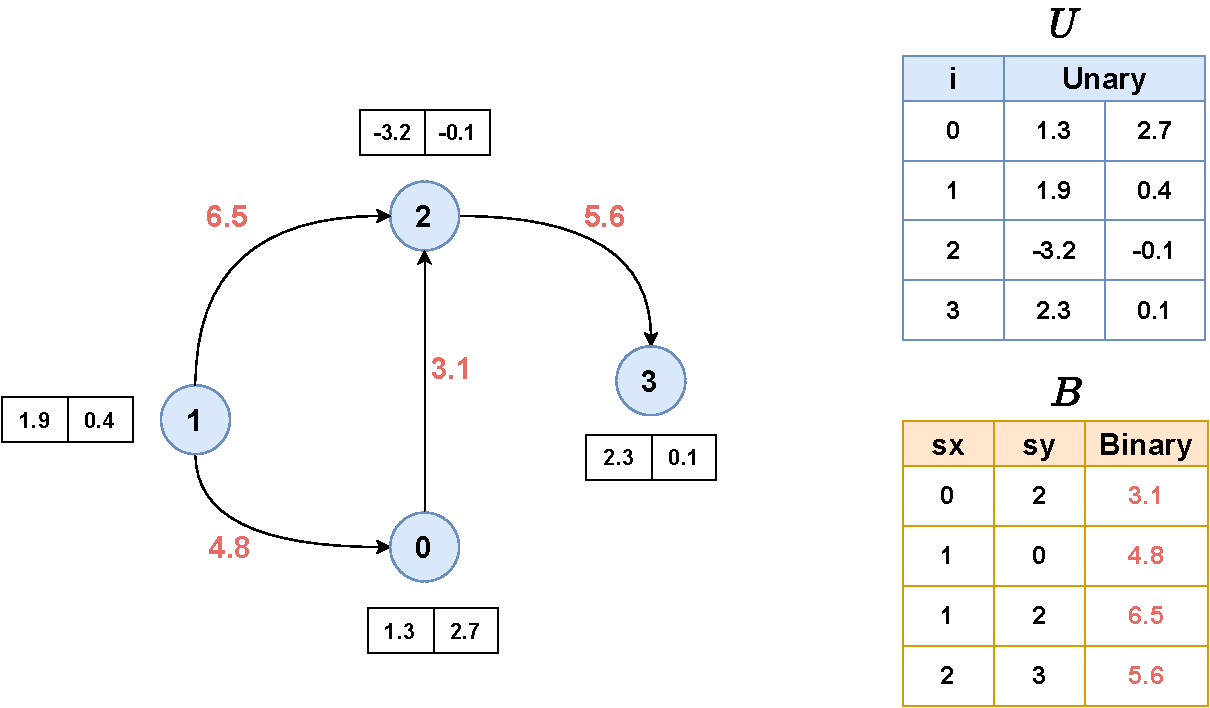
\includegraphics[width=0.7\linewidth]{figures/kenn_relational_representation2.pdf}
 	\caption{Representation of relational data inside KENN. Specifically, objects and relations can be seen as nodes and edges of a directed graph. The preactivations of each grounded predicate are represented in tables $U$ and $B$. In this example, two unary predicates and one binary predicate are present. Note that in matrix $B$ only the object pairs such that there is a relation between them are reported.}
 	\label{fig:KENNrelationalrepr}
 \end{figure}

\subsubsection{The JOIN operation}
At this stage, we have two matrices, $U$ and $B$, containing preactivations of unary and binary predicates respectively. However, recall that the CE module takes in input a single matrix containing all the preactivations, in order to compute the deltas. The fact is that, given any binary clause, we must be able to access the preactivation value of any of its atoms, from a single matrix. Take as an example the grounded clause $A(c_1) \vee B(c_1,c_2) \vee \neg A(c_2)$. The preactivations of $A(c_1)$ and $ A(c_2)$ can be accessed from matrix $U$, but the one for $B(c_1, c_2)$ can be accessed only from $B$.
For this reason, we need a way to merge both the binary and unary preactivations into a single matrix. KENN does this with the JOIN operation. 
%Specifically, when using $n$ unary predicates 
%%$\{U_1,\dots, U_n\}$ 
%and $m$ binary predicates 
%%$\{B_1, \dots, B_m\}$
%, the JOIN operation is defined as follows:
\begin{definition}[JOIN]
	Given $n$ unary predicates, $m$ binary predicates and their respective matrices $U$ and $B$, the JOIN operation is defined as follows:
	\begin{equation*}
	\operatorname{JOIN}(U,B) = M
	\end{equation*}
	where the $i$-th row of the matrix $M$ is:
	\begin{equation*}
	\begin{align*}
	&M_{i} = (s^x,s^y, U_{s^x2}, \dots, U_{s^x(n+1)}, U_{s^y2}, \dots, U_{s^y(n+1)},B_{i3},\dots, B_{i(m+2)}),\\
	&\text{where   } s^x = B_{i1}, s^y = B_{i2}.
	\end{align*}
	\end{equation*}
More simply, $M$ has the same number of rows as matrix $B$ and shares its two first columns; additionally, it also contains the preactivations of all the unary predicates for both the first and second index of each row, together with all the preactivations for the binary predicates. 
\end{definition}

From this new matrix, the CE can access the preactivations for any atom of any grounded binary clause and can compute a delta matrix, which we will call $\delta M$.


\subsubsection{The GROUP BY and SELECT operations}
As we saw with our previous example, binary clauses can also contain unary predicates. This implies that the delta vectors generated from binary clauses can actually modify the preactivations of both unary and binary predicates. More specifically, this means that the matrix $\delta M$ contains some information that is supposed to go both inside matrices $\delta U$ and $\delta B$. KENN extracts the unary deltas from $\delta M$ with the GROUP BY operation, and does the same for the binary deltas with the SELECT operation.

\begin{definition}[GROUP BY]
	The GROUP BY ($\text{GB}$) operation takes in input the matrix of deltas $\delta M$ and an index ($x$ or $y$), and is defined as follows:
	\begin{equation*}
	\begin{cases}
	\operatorname{GB}(\delta M, x)= \delta U_x\\
	\operatorname{GB}(\delta M, y)= \delta U_y,
	\end{cases}
	\end{equation*}	
	where 	
	\begin{equation*}
	\begin{cases}
	\left(\delta U_x \right)_i = \left(i, \sum_{j\in J^i_x}\delta M_{j3},\dots, \sum_{j \in J^i_x}\delta M_{j(2+n)}\right)\\
	\left(\delta U_y \right)_i = \left(i, \sum_{j\in J^i_y}\delta M_{j(n+3)},\dots, \sum_{j \in J^i_y}\delta M_{j(2n+2)}\right)\\
	J^i_x:=\{j:\delta M_{j1}=i\}\\
	J^i_y:=\{j:\delta M_{j2}=i\}.
	\end{cases}
	\end{equation*}
\end{definition}
In simple terms, the GROUP BY operation extracts the deltas for the unary predicates from the delta matrix $\delta M$, by aggregating the results for each object identifier. This is exactly equivalent to a GROUP BY query in a relational database.

\begin{definition}[SELECT]
The SELECT operation simply extracts the deltas for the preactivations of the binary atoms from the $\delta M$ matrix. Specifically:
$$\operatorname{SELECT}(\delta M) = \delta B $$
where:
$$\delta B_i = \left(\delta M_{i1}, \delta M_{i2}, \delta M_{i(2n+3)},\dots, \delta M_{i(2n+m+2)}\right).$$
\end{definition}

\subsubsection{Computing the delta matrices} 

Now that all the necessary tools have been defined, we are ready to describe the process to compute the matrices $\delta U$ and $\delta B$. KENN uses two different KEs to generate delta matrices: one ($\text{KE}_u$) takes in input the matrix $U$, and returns a delta matrix $\delta U_u$, using the standard procedure for unary predicates described in the previous section. The other ($\text{KE}_b$) takes in input a matrix $M=\text{JOIN}(U,B)$, and returns a delta matrix $\delta M$. Afterwards, the following operations are performed:
\begin{enumerate}
	\item The final delta matrix for binary predicates is obtained as follows: $\delta B = \operatorname{SELECT}(\delta M)$;
	\item Two matrices $\delta U_x = \operatorname{GB}(\delta M, x)$ and $\delta U_y = \operatorname{GB}(\delta M, y)$ are computed;
	\item $\delta U_x$ and $\delta U_y$ are summed together, obtaining matrix $\delta U_b$;
	\item The final delta matrix for unary predicates is obtained as follows: $\delta U = \delta U_u + \delta U_b$.
\end{enumerate}
In Figure \ref{fig:kenn_rel_global_scheme}, we report an example with the whole process.


\begin{figure}
	\centering
	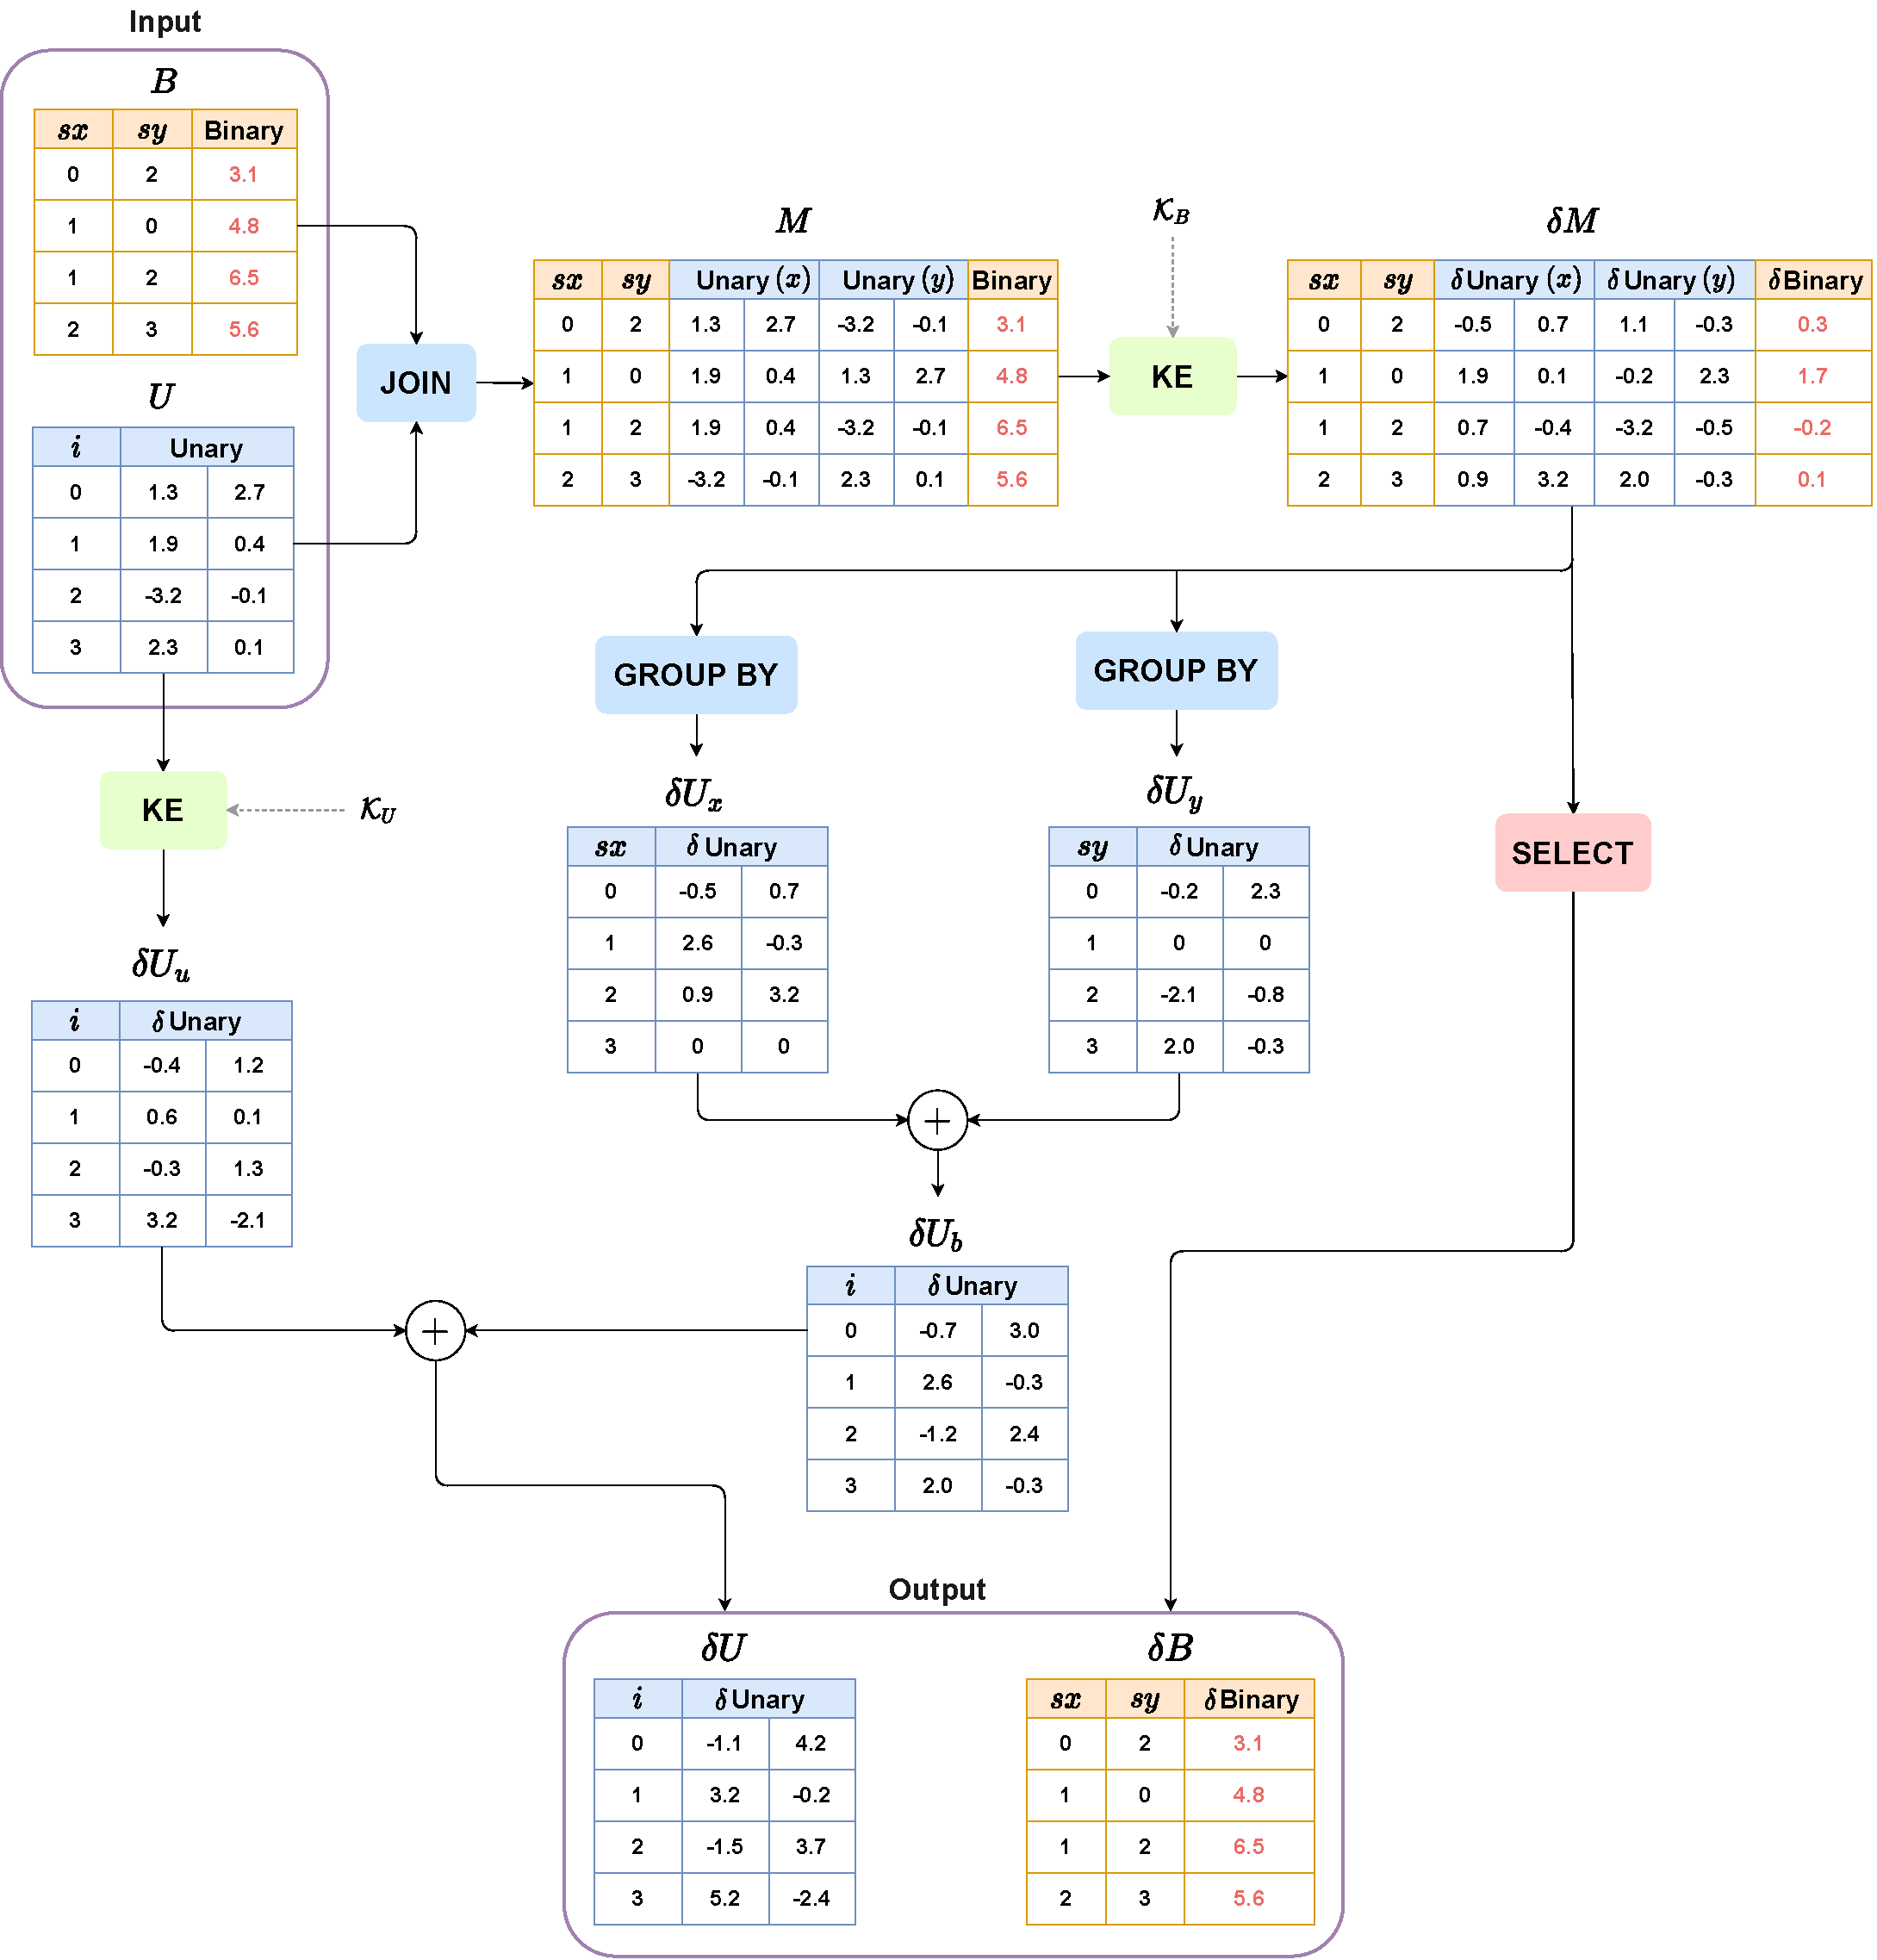
\includegraphics[width=\linewidth]{figures/kenn_relational_global_chart.pdf}
	\caption{This figure shows an example with all the necessary computations to compute the final delta matrices $\delta U$ and $\delta B$ (in the bottom), starting from matrices $U$ and $B$ (top left).}
	\label{fig:kenn_rel_global_scheme}
\end{figure}
 
 
 \section{Related Work}
 As already introduced at the end of Chapter \ref{chapt:explainability}, the integration of statistical learning with logical symbolic knowledge is one of the key challenges in the research on artificial intelligence, specifically for the field of NeSy. Authors of \cite{daniele2019kenn} subdivide NeSy sytstems into three main groups, based on their different objectives:
 \begin{enumerate}
 	\item \textbf{Differentiable Reasoning }: in this category, the goal is to create differentiable approaches for deductive resoning, which can be defined as the process of producing logical deductions from an initial knowledge base;
 	\item \textbf{Inductive Logic Programming} : here the goal is to extract logical knowledge from data, or to refine an existing one;
 	\item \textbf{Knowledge Guided Learning}: here the goal is learning in classical ML sense, where the knowledge has the role of a supervisor, meaning that the machine should learn according to the base knowledge.
 \end{enumerate}

 We are interested in Knowledge Guided Learning (KGL), the class of models where KENN belongs. The objective is to improve the performance of a NN model, by providing a Prior Knowledge which is expressed in terms of logical formulas and which acts as a supervisor for the learning process. At present, two main ways of injecting knowledge inside NN have been employed. The first one involves the usage of a regularization term in the loss function. Indeed, logical rules can be interpreted as constraints for the weights in the learning process; in ML, the natural way to introduce constraints in learning is to add a penalization term in the loss function, which represents in some way the satisfaction of the logical rules. The second approach, adopted by KENN, is to directly modify the network architecture: in this way, logical rules are enforced at the level of the network topology.
 
 \subsection{Regularization Approaches}
In KGL, regularization approaches enforce the satisfaction of the knowledge by defining a special penalization term to be applied to the loss function. Here we briefly mention two important examples of regularization based approaches: Logic Tensor Networks and Semantic Based Regularization.
 
 \subsubsection{Logic Tensor Networks}
 Logic Tensor Networks (LTN) \cite{serafini2016logic} is a notable example of a method capable of integrating logical knowledge inside a NN by directly modifying the loss function. To do this, the authors define a differentiable first-order logic language called Real Logic, with which they manage to represent common deep learning tasks, such as clustering, multi-label classification, relational learning, regression, embedding learning and many others. 
 %LTN can also perform reasoning, which is the task of verifying if a formula is a logical consequence of another formula. 
 In simple terms, the role of Real Logic is to act as a bridge between the purely symbolic world of logic, and the sub-symbolic world of neural systems. 
This is achieved by defining a specific semantic for the language, where each domain is interpreted as sets of tensors in the real field. In the same way, each constant, variable and term of the language is interpreted as a tensor of real values, function symbols are interpreted as functions between tensors, and predicates are interpreted as functions that map tensors into the interval $[0,1]$. Specifically, given $s$ any symbol of the language $\mathcal{L}$, the authors call its interpretation the \say{grounding} of $s$, and denote it with $\mathcal{G}(s)$\footnote{Note how here the term \say{grounding} differs from the standard meaning, which was defined in Section \ref{sec:kenn_theoretical_framework}. While talking about LTN, the term \say{grounding} should be read as \say{interpretation}.}.
 
% Real Logic is defined over a first order language $\mathcal{L}$ with a signature containing a set of constant symbols (or objects) $\mathcal{C}$, a set of variable symbols $\mathcal{X}$, a set of functional symbols $\mathcal{F}$ and a set of relational symbols (or predicates) $\mathcal{P}$. We refer to the set $\mathcal{S} = \mathcal{C} \cup \mathcal{X} \cup \mathcal{F} \cup  \mathcal{P}$ as the set of symbols of $\mathcal{L}$. Each symbol of the language can belong to different domains (i.e. can be of different types): for example the constant $c_1 \in \mathcal{C}$ can represent a specific person, while the constant $c_2 \in \mathcal{C}$ can represent a specific city. The same concept applies to functions and predicates. To represent the domain of each symbol, it is assumed that there exists a non-empty set $\mathcal{D}$, containing all the domains, which are in turn symbols. Then, to properly assign each symbol to its corresponding domain, the functions $\mathbf{D}, \mathbf{D_{in}}$ and $\mathbf{D_{out}}$ are defined:
% \begin{equation*}
% \mathbf{D}: \mathcal{X} \cup \mathcal{C} \rightarrow\mathcal{D}
% \qquad \qquad
% \mathbf{D_{in}}: \mathcal{F} \cup \mathcal{P} \rightarrow\mathcal{D^*}
% \qquad \qquad 
% \mathbf{D_{out}}: \mathcal{F} \rightarrow\mathcal{D},
% \end{equation*}
% where $\mathcal{D^*}$ is the set of all finite sequences of symbols in $\mathcal{D}$.
% %The set of terms of the language $T$ is recursively defined, to be the smallest set such that...
% The point where the symbolic language meets the subsymbolic world of neural networks is in the definition of grounding, which is the process in which each symbol is given its numeric representation. Indeed, in Real Logic, each domain is interpreted as sets of tensors in the real field. In the same way, each constant, variable and term of the language is interpreted as a tensor of real values, and function symbols are interpreted as functions between tensors. 
 %By defining how to apply the grounding for each symbol of $\mathcal{L}$, semantic of $\mathcal{L}$. 
 The authors then define how to compute the grounding of formulas, by using the semantics of first-order fuzzy logic. 
 The way in which learning becomes possible is by defining the parametric grounding for symbols: given a symbol $s$, the parametric grounding of $s$ is a grounding which is not known in advance, and can be computed exclusively by knowing a set of parameters. It is denoted as $\mathcal{G}(s|\theta_s)$, where $\theta_s$ is the set of parameter values that uniquely determines the value of the grounding. 
With this setup, learning is defined as the process of searching for the set of parameters $\theta^*$ such that:
 	\begin{equation*}
 	\theta^{*}=\underset{\theta \in \Theta}{\operatorname{argmax}} \left(\underset{\phi \in \mathcal{K}} {\operatorname{SatAgg}} \mathcal{G}_{\theta}(\phi)\right),
 	\end{equation*} 
 where the quantity $\underset{\phi \in \mathcal{K}} {\operatorname{SatAgg}} \mathcal{G}_{\theta}(\phi)$ denotes the level of satisfiability of all the formulas in the knowledge base, with respect to a given aggregating operator $\operatorname{SatAgg}:\left[0,1\right]^* \rightarrow \left[0,1\right]$, which has the task of aggregating all the truth values of the formulas.

 
 It's interesting to note that, based on what kind of symbol we are learning the grounding for, one can identify a corresponding task in machine learning:
 \begin{itemize}
 	\item If $s \in \mathcal{C}$, corresponds to learning an embedding;
 	\item If $s \in \mathcal{F}$, it corresponds to learning regression tasks;
 	\item If $s \in \mathcal{P}$, it corresponds to learning a classification task.
 \end{itemize}
For the simple case of binary classification, for example, the task is to learn the parametric grounding of a predicate $A$, $\mathcal{G}(A|\theta):x \rightarrow \sigma(\operatorname{MLP}_{\theta}(x))$, where $\operatorname{MLP}$ denotes a multi layer perceptron. If we define with $D$ the dataset with all the examples, the actual loss function to minimize will be:
	\begin{equation*}
	L = \left(1 - \underset{\phi \in \mathcal{K}} {\operatorname{SatAgg}} \mathcal{G}_{\theta,x\leftarrow B}(\phi(x)) \right),
	\end{equation*}
	where the notation $\underset{\phi \in \mathcal{K}} {\operatorname{SatAgg}} \mathcal{G}_{\theta,x\leftarrow B}(\phi(x))$ means that the variable $x$ is grounded with the data $B$, where $B$ is a mini-batch sampled from $D$. 
	Note how LTN does not define a regularization term to add to a predefined loss function, but defines the entire loss in terms of satisfiability of formulas. This means that also the supervised learning paradigm is enforced by logical rules. More specifically, for the case of binary classification, for each sample $a$ belonging to the positive class, the knowledge base will contain the formula $P(a)$, where the atom $P(a)$ means \say{sample $a$ belongs to the positive class}. The same happens for all the representatives of the negative class.

 
 \subsubsection{Semantic Based Regularization}
 Semantic Based Regularization (SBR) is a general learning framework designed to integrate domain specific background knowledge in the form of first-order logic (FOL) clauses. To enforce the satisfaction of all the clauses, SBR introduces special regularization terms in the loss function, which represent the satisfaction of the knowledge. Specifically, given a background knowledge represented by set of $H$ clauses, the satisfaction of the $h$-th clause can be represented by the quantity denoted by $0 \leq \phi_h(f) \leq 1$, where $f$ is the vector of predictions provided by the model. From here, the regularization term to be added to the loss function is defined as
 $$ \sum_{h=1}^H \lambda_h(1 - \phi_h(f)), $$
 where $\lambda_h$ is the weight associated to the $h$-th constraint. A higher value of $\lambda_h$ will increase the cost of not satisfying the constraint, meaning that the importance of the corresponding rule will increase. The conversion of FOL clauses into differentiable functions is made possible by considering fuzzy generalizations of FOL logic, similarly to how it is done in KENN. This is a natural approach for machine learning tasks, but a major disadvantage over KENN is that, since the clause weights are introduced at the level of the loss function, those cannot be learned and are required to be known in advance. This, of course, is unlikely to happen in real scenarios and it is much more desirable to learn the weights together with the other learnable parameters of the model.
 
 \subsection{Model Based Approaches}
 An example of model based approach for the integration of logic in NNs is represented by Relational Neural Machines (RNM) \cite{marra2020relational}. A RNM models a probability distribution over a set of $m$ output variables, given the predictions provided by one (or more) base NN, and a set of model parameters. Specifically, differently from a standard NN, each forward pass in RNM is performed in two separate stages: in the first one, the predictions from the NN are obtained from the input data; the second is a \textit{semantic} stage, where the logical costraints are enforced over the output. More precisely, this second stage is performed by an undirected graphical model.
 RNM defines a conditional probability distribution of the exponential family over the output variables, which is defined as follows:
 \begin{equation*}
 p(y|f,\lambda) = \frac{1}{Z} \exp \left( \sum_{x \in S}\Phi_0(f(x),y(x))+\sum_c \lambda_c \Phi_c(y) \right), 
 \end{equation*}
 where $Z$ is the partition function, $f(x)$ are the predictions from the NN, $\lambda$ is the set of parameters driving the semantic stage, $\Phi_0$ is a potential function which enforces the supervised learning paradigm, $S$ is the subset of supervised input vectors and $\Phi_c$ is a potential associated to $c$, a FOL formula part of the base knowledge. Specifically, $\Phi_c$ enforces the satisfaction of the clause $c$, while $\lambda_c$ determines the weight of such clause. 
 
 The approach used by RNM is similar to the one used in KENN: a base NN (or any learner) is used as a foundation which provides initial predictions: on those, the model performs a post elaboration step, enforcing logical rules and improving the predictions. Also, like in KENN, the clause weights are trained together with the whole model, which is a desirable thing in real use cases. However, one significant drawback of RNM is that, for each training step, and also at inference time, an optimization problem must be solved. 
Specifically, the best assignment for the output variables is found with a Maximum a Posteriori (MAP) estimation, which maximizes the posterior probability of the grounded target variables, given the predictions from the base NN and the parameters $\lambda$:
 \begin{equation*}
 y^* = \underset{y}{\operatorname{argmax}}P(y|f,\lambda).
 \end{equation*}
 In comparison, KENN is much more efficient since it is implemented as an actual layer of the NN architecture, which is then trainable end-to-end, together with the clause weights.
 
 
 
 \section{Experiments}
 \label{sec:kenn_experiments}
 
In this section we describe in detail the experiments performed with KENN. We tested the ability of KENN of working with relational data, in the context of Collective Classification~\cite{sen2008collective}, both with the inductive and transductive learning paradigm. 

\begin{definition}[Collective Classification]
Consider a directed graph, consisting in a set of nodes $V$ and a set of edges $E$. Each $v \in V$ is described with a vector of features $x\in \mathbb{R}^n$ and belongs to one of $k$ classes $\{\omega_i\}_{i=1}^k$. The set of nodes $V$ is further divided in two subsets of nodes: $X$, the set of nodes for which the correct label is known (Training Set), and $Y$, the set of nodes for which it is unknown (Test Set). The task of Collective Classification is to correctly predict the labels of nodes in $Y$, given the feature vectors of $X$ and the topology structure determined by $E$. 
\end{definition}
Two learning paradigms can be defined:

\begin{itemize}
	\item \textbf{Inductive Learning}: two separate graphs are used: $G_x = (X,E_x)$ for training and $G_y = (Y, E_y)$ for testing, where $E_x = \{(u,v) | u,v\in X\}$ and $E_y = \{(u,v) | u,v\in Y\}$. In other words, the edges of nodes between train and test set are not considered.
	\item \textbf{Transductive Learning}: a single graph is considered, with both training and test nodes: the network can use the information coming from the relations from the Test set even during training, but the actual supervision will come only from training nodes. Compared with the inductive paradigm, here the network has more available information, and for this reason we can expect better results.
\end{itemize}

We also provide a comparison of our results with the ones from SBR and RNM, reported on \cite{marra2020relational}, on the same dataset and using the same learning paradigms. All the experiments were carried out with Python 3 and TensorFlow 2 \cite{abadi2016tensorflow}. All the code is publicly available on Github\footnote{\url{https://github.com/rmazzier/KENN-Citeseer-Experiments}}.

\subsection{Citeseer Dataset}

The experiments were conducted on the Citeseer Dataset \cite{lu2003link}: it consists in a citation network with $4732$ citations (directed links) between $3312$ scientific publications (nodes), belonging to $6$ different classes which represent the topic of the paper. Each node in the dataset is represented by a $0/1$ valued feature vector, where each entry indicates the absence or presence of the corresponding word in the dictionary, which is constituted by $3703$ unique words.

\subsection{The Prior Knowledge}

The knowledge that we want to use in order to improve the predictions from the NN is the intuitive fact that, if a paper cites another paper, it is probably true that they are of the same topic. If we denote with $T_i(x)$ the truth value that node $x$ belongs to the $i$-th output class, this fact can be encoded in terms of a logical clause as follows:
$$\forall x \forall y \quad T_i(x) \wedge \operatorname{Cite}(x, y) \rightarrow T_i(y), \quad i=1,\dots,6$$
meaning that the this clause is repeated one time for each different output class. Inside KENN, this clause is represented as a disjunction of literals as follows:

$$\forall x \forall y \quad \neg T_i(x) \vee \neg \operatorname{Cite}(x,y) \vee T_i(y), \quad i=1,\dots,6 $$

\subsection{Experimental Setup}
%TODO: rephrase..
The aim of these experiments was to obtain comparable results to those reported in \cite{marra2020relational}. For this reason we used the same base NN that was used there, which consists in a fully connected dense NN with three hidden layers, each of which using $50$ hidden units and the ReLu activation function. Specifically, the NN takes in input only the features of each document in the dataset, meaning that it will be blind to the relations between them. For this reason, we can already observe that the predictions of the NN will not be influenced in any way by the choice of the learning paradigm. Specifically, we used the same random seed for both the tasks, so the the predictions of the NN are exactly the same between the two paradigms.
The relational information (i.e. the citations between the papers) is introduced only at the level of the KE, and is treated as base knowledge. Note that this is a very specific case: KENN, in general, is designed to be able to learn both unary and binary predicates. In this case instead, the relational knowledge is provided as ground truth and is used as an additional piece of information, which is exploited by the model to produce better predictions. Also note that the only learned predicates are the unary ones. Specifically, the forward pass is constituted by the following steps:
\begin{enumerate}
	\item The base NN takes in input the matrix of features for the current batch of data, and returns the matrix of unary preactivations $U$ (without the column containing the object identifiers, which is left implicit);
	\item The matrix of binary predicates $B$ is derived directly from the data, according to the current learning paradigm being considered. Since there is just a binary predicate, namely the $\operatorname{Cite}$ predicate, matrix $B$ will have just three columns, two for the indices of the object pairs, and one for the truth value of the binary predicate. 
	\item KENN takes in input $U$ and $B$, and produces deltas $\delta U$ and $\delta B$, as described in Section \ref{sec:relational_kenn}. Since we are just interested in learning unary predicates, we just keep $\delta U$, while $\delta B$ is discarded;
	\item Differently from the standard case where the sigmoidal activation function is applied in the KE module, here the KE uses the softmax activation function. This is because for these experiments we are considering a multi-class classification task where each object can belong exclusively to one class. Specifically, the output of the KENN layer is obtained as follows:
	\begin{equation*}
	y'= \operatorname{softmax}(U + \delta U).
	\end{equation*}
	
\end{enumerate}

In Figure \ref{fig:citeseer_setup_chart} an example with all the listed steps is reported.
Additionally, note that the truth values of the connections for this dataset are hard, meaning that nodes can be either connected or not connected, with no other alternative. For this reason pairs of connected objects are assigned a very high value, in this case $500$\footnote{There is not a specific reason for the choice of this number. The only important thing is that, when applying the sigmoidal activation function, the resulting truth value is close to $1$.}. Also notice that only the pairs of connected objects are reported in $B$. In fact, it would be useless to consider also the pairs of not connected nodes (thus having a preactivation value equal to $-500$ for the $\operatorname{Cite}$ predicate), since for those cases the grounded clauses of our knowledge would be automatically satisfied\footnote{Take $c_1$ and $c_2$ two nodes in the graph which are not connected; given the clause $\neg T(c_1) \vee \neg \operatorname{Cite}(c_1,c_2) \vee T(c_2)$, its truth value will be always $\approx 1$, since $\mathcal{I}(\neg \operatorname{Cite}(c_1,c_2)) \approx 1$. }, and KENN would not apply any change. Thus, the number of rows of matrix $B$ will be equal to the number of edges in the training graph.

%TODO continua qui
In our model architecture, we also stack three KENN layers instead of only one: this choice is motivated by the fact that a single layer would consider only the neighbors of each node. By adding three layers, instead, we allow for a propagation of the changes to farther nodes. This intuition was confirmed by empirically better results with respect to ones using a single KENN layer.

In addition to considering two different learning paradigms, we also evaluate our model on splits of different sizes, in order to see the impact of the dataset size on the final results. Specifically, for each learning paradigm, the model is trained on $10\%$, $25\%$, $50\%$, $75\%$, $90\%$ splits of the whole dataset. Additionally, to have statistically relevant results, for each training percentage the dataset was trained for $500$ times, where each time the training data is randomly picked in such a way that the class balance between train validation and test sets is preserved. Such a high number was motivated by the fact that, when training on always different splits, variance of the results can be very high, especially in the cases where the training set constitutes a small percentage of the whole dataset. In \cite{marra2020relational}, the same procedure has been adopted, with the only difference that the number of training runs for each split percentage was $10$ instead of $500$. This was probably due to much longer training times: recall that in the case of RNM an optimization problem must be solved at each training step and also at inference time. Indeed, this fact highlights how one of the main advantages of KENN is its efficiency and scalability. Due to the different number of training runs, results won't be exactly comparable to the ones provided in \cite{marra2020relational}; nevertheless, our results will have a strong statistical significance. Additionally, we also provide $95\%$ confidence intervals for each test set accuracy, as well as \mbox{p-values} with respect to the null hypothesis that the mean test set accuracy of KENN is the same as the one of the base NN.

\begin{figure}
	\centering
	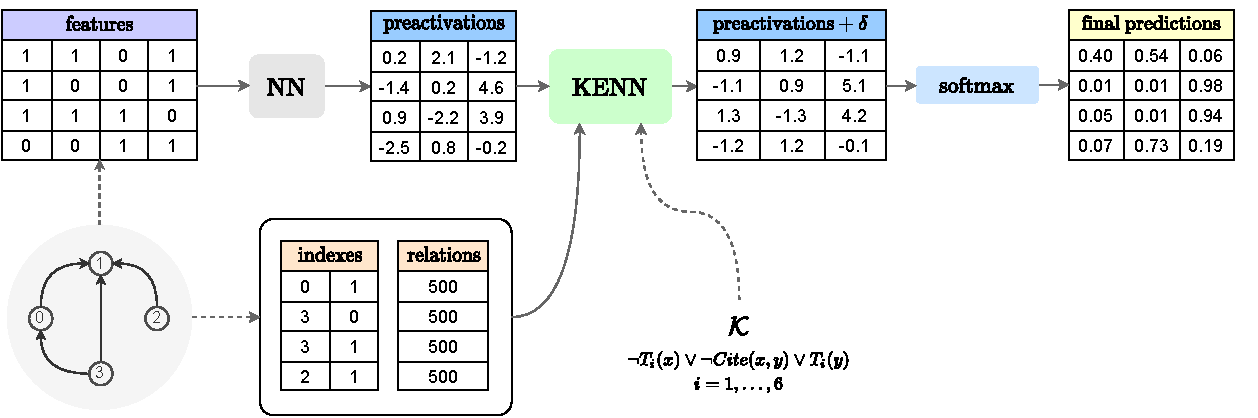
\includegraphics[width=\linewidth]{figures/citeseer_setup.drawio.pdf}
	\caption{Simple example showing how the relational knowledge is injected in the NN for the Citeseer experiments. In this toy example, features are $4$-dimensional vectors and there are $3$ unary predicates; in the actual experiments, feature vectors have $3703$ components and the output classes are $6$.}
	\label{fig:citeseer_setup_chart}
\end{figure}


\subsection{Results}
\subsubsection{Inductive Learning}

In Table \ref{tab:resultsinductive} we report the results of the experiments for the inductive case. Specifically, each column contains the mean of all the test set accuracies from the different runs. The results for SBR and RNM are the ones reported in \cite{marra2020relational}. Also note that since we were not able to perfectly replicate the results for the base NN accuracies reported in \cite{marra2020relational}, we report the ones obtained by our base NN, and use the relative improvements as the main evaluation metric.
The relative improvements are also visualized in Figure \ref{fig:inductive_deltas_comparison}, together with $95\%$ confidence intervals, with a comparison with those from SBR and RNM. Finally in Figure \ref{fig:inductive_histograms}, we report histograms showing the distribution of the test set accuracies of both our base NN and KENN, together with the distribution of the relative improvements for all the runs.
The p-values for every training percentage were extremely small and well below the $0.05$ threshold: for completeness, they are reported in Table \ref{tab:p_vals}. This means that, for both the training paradigms, we can safely reject the null hypothesis and be almost sure that the improvements provided by KENN are not a result of random perturbations due to the different choice of the training splits.
\begin{table}[h]
	\caption{Test set accuracies obtained with the inductive paradigm. The columns for SBR and RNM show the results reported in \cite{marra2020relational}. The quantities between parentheses denote the relative improvement with respect to the base NN.}
	\label{tab:resultsinductive}
	\centering
	\scalebox{0.95}{
	\begin{tabular}{c|lll|ll} 
		\% training & NN & SBR & RNM & NN & KENN \\
		\hline 
		\rule{0pt}{3ex}    $10$ & $0.645$ & $0.650$ & $\mathbf{0 . 6 8 5}$ & $0.544$ & $0.601$ \\
		& & $(+0.005)$ & $(+0.040)$ & & $\mathbf{(+0.048)}$ \\
		$25$ & $0.674$ & $0.682$ & $\mathbf{0 . 7 0 9}$ & $0.629$ & $0.671$ \\
		& & $(+0.008)$ & $(+0.035)$ & & $\mathbf{( + 0 . 0 4 1 )}$ \\
		$50$ & $0.707$ & $0.712$ & $\mathbf{0 . 7 2 6}$ & $0.680$ & $0.714$ \\
		& & $(+0.005)$ & $(+0.019)$ & & $(+\mathbf{0 . 0 3 4 )}$ \\
		$75$ & $0.717$ & $0.719$ & $0.726$ & $0.733$ & $\mathbf{0 . 7 5 4}$ \\
		& & $(+0.002)$ & $(+0.009)$ & & $\mathbf{( + 0 . 0 2 1 )}$ \\
		$90$ & $0.723$ & $0.726$ & $0.732$ & $0.759$ & $\mathbf{0 . 7 6 8}$ \\
		& & $(+0.003)$ & $(+0.009)$ & & $\mathbf{( + 0 . 0 1 0 )}$\\	
		\hline \hline
	\end{tabular}}
\end{table}
\begin{figure}
	\centering
	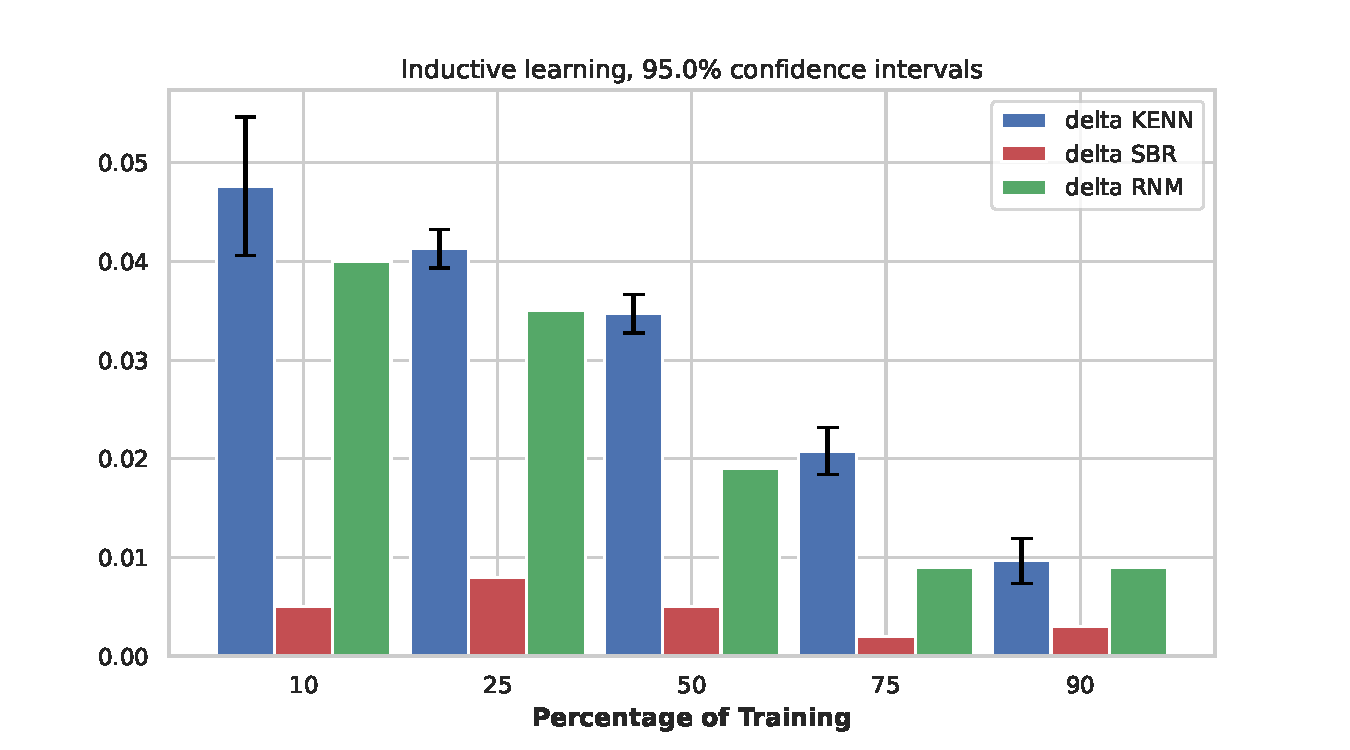
\includegraphics[width=0.8\linewidth]{figures/deltas_inductive.pdf} 
	\caption{Relative improvements for the inductive learning task. $95\%$ confidence intervals are provided for our results.}
	\label{fig:inductive_deltas_comparison}
\end{figure}
\begin{figure}
	\centering
	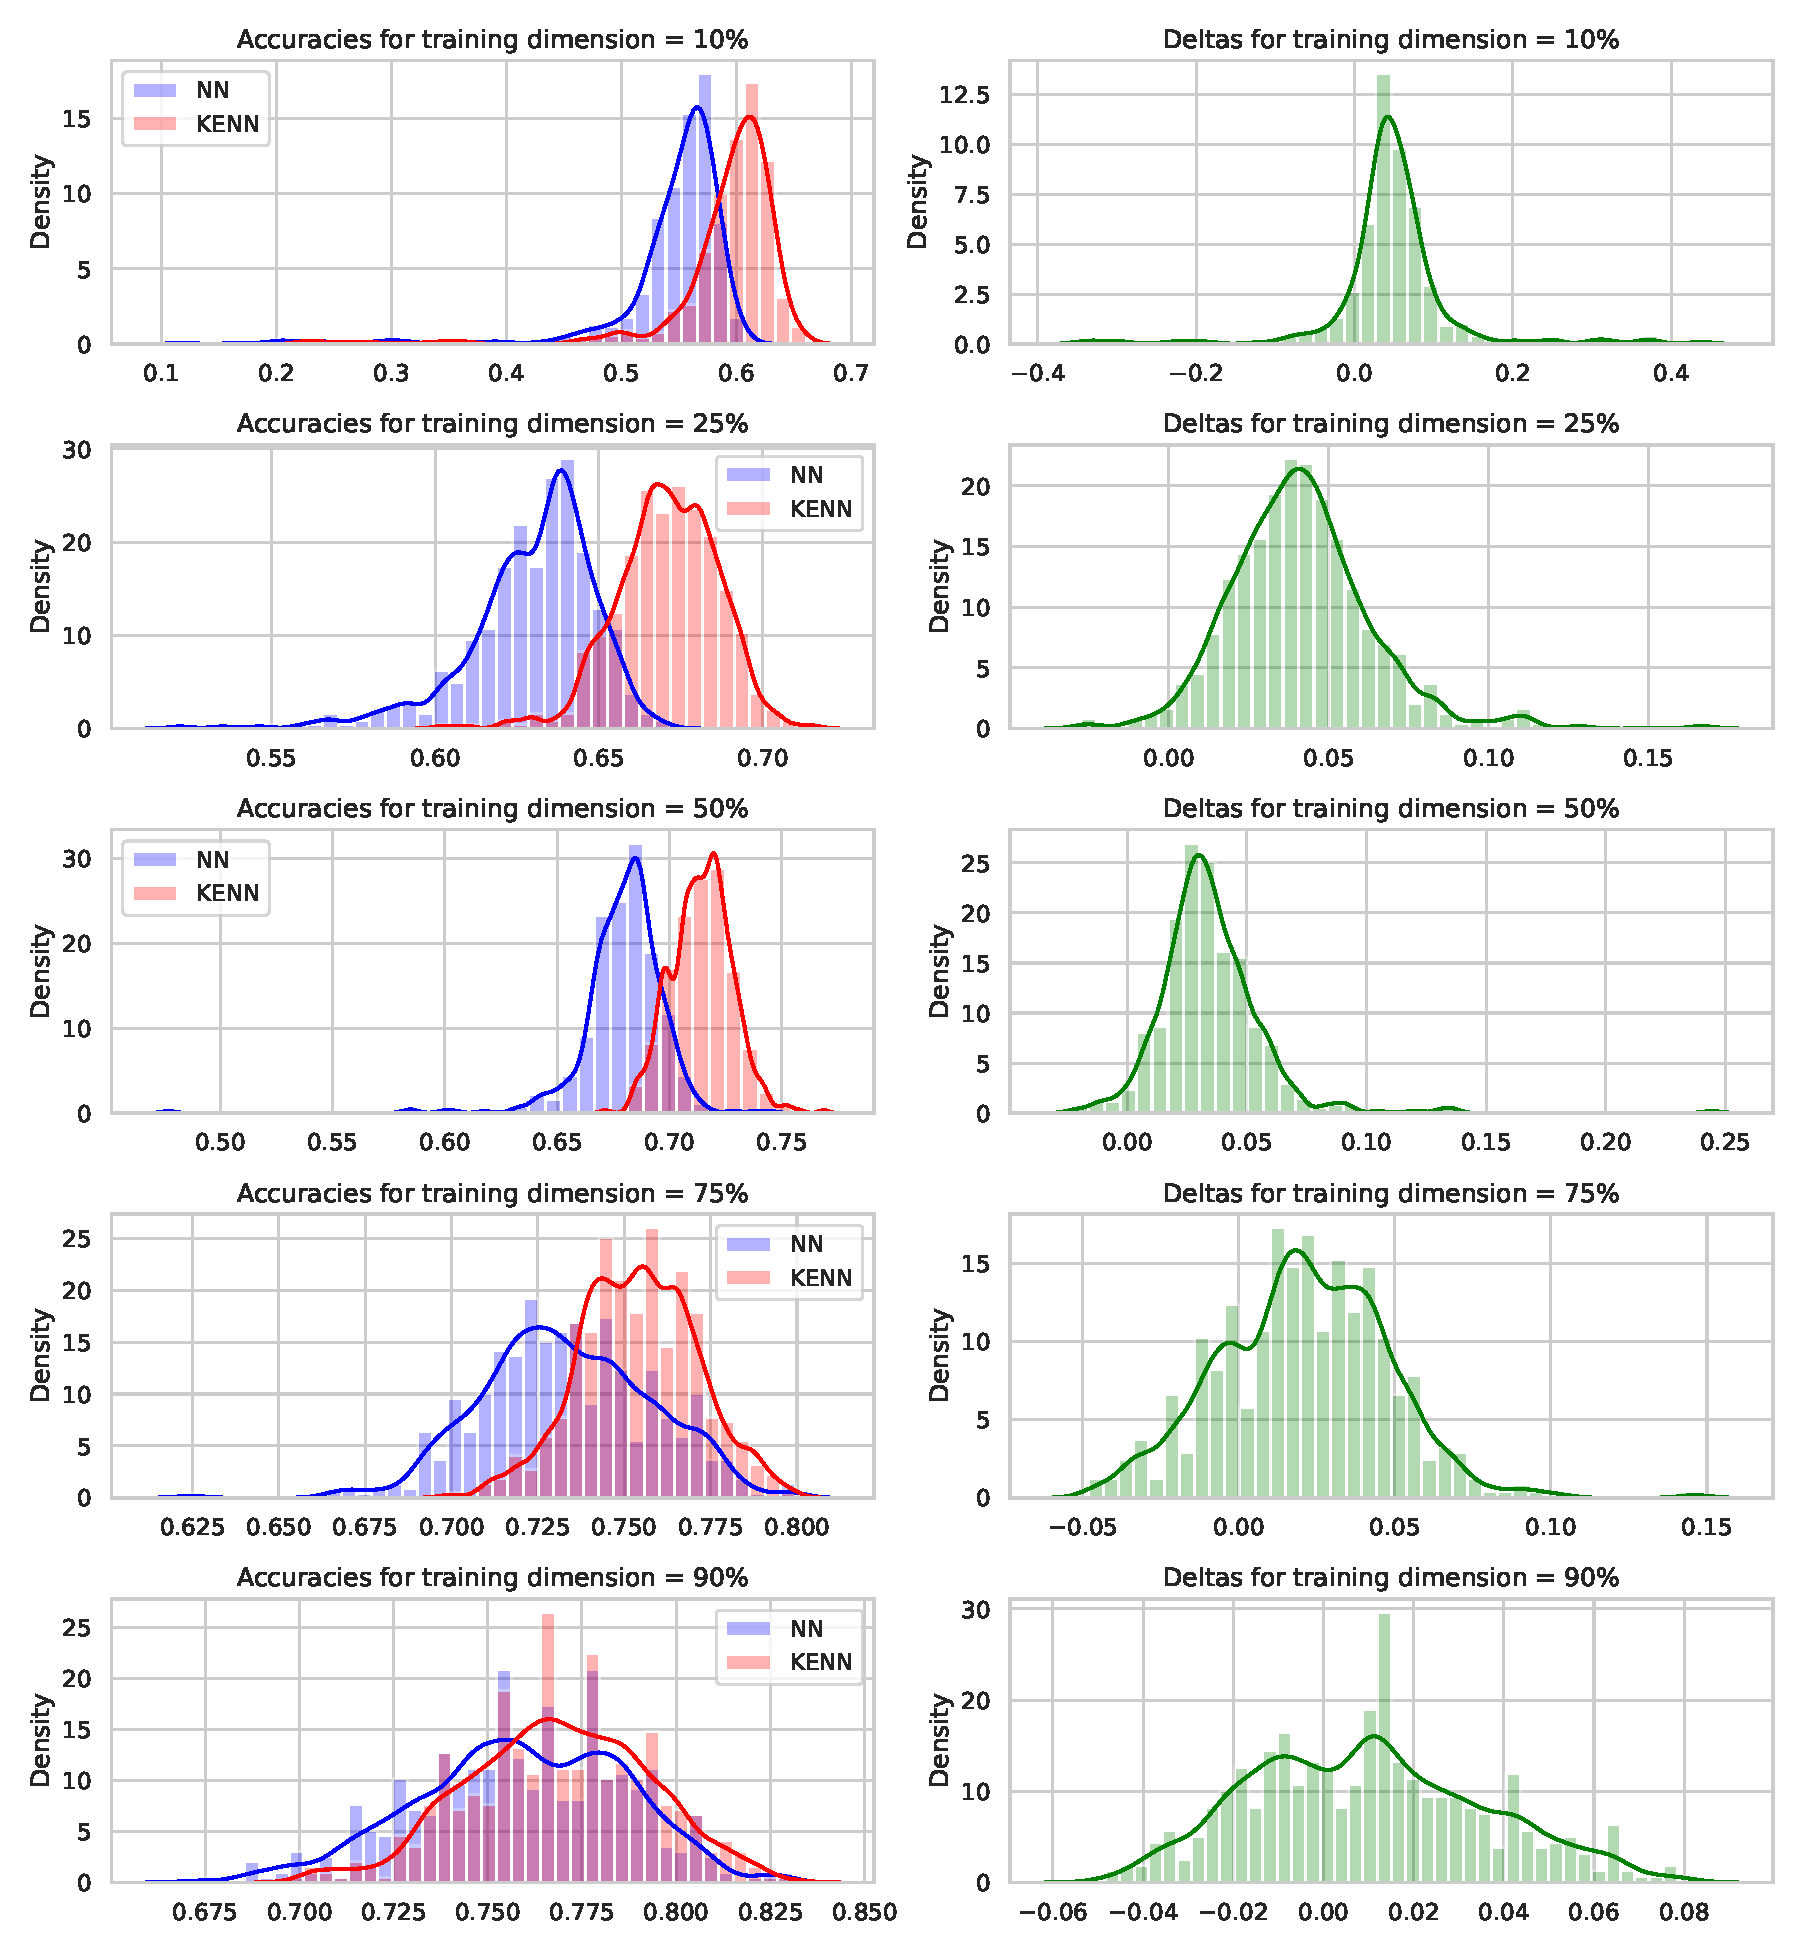
\includegraphics[width=0.95\linewidth]{figures/histograms_inductive.pdf}
	\caption{Histograms showing the distribution of the accuracies for all the different $500$ runs, for the inductive case. On the left, the accuracies of the base NN vs accuracies of KENN. On the right the distribution of the relative improvements.}
	\label{fig:inductive_histograms}
\end{figure}
As we can observe, KENN outperforms both RNM and SBR for each training percentage. Additionally, we can see how the relative improvement becomes smaller as the training percentage increases. This makes sense from an intuitive point of view: when disposing of few data, NNs struggle to give good results and the prior knowledge plays a more important role, providing more improvements. On the other hand, when the NN is trained on a lot of data, the knowledge becomes less important: indeed the NN has now access to much more information and, in some sense, can learn the rules on its own from the patterns in the data. In this sense, RNM shows a similar behavior with respect to KENN, even if providing less relative improvement overall.

\subsubsection{Transductive Learning}

We report the same results for the transductive case in Table \ref{tab:resultstransductive}, Figure \ref{fig:transductive_deltas_comparison} and Figure \ref{fig:transductive_histograms} respectively. Note that the results of our NN are exactly same of the ones from the inductive paradigm; this is because we used the same random seed for both the paradigms, and, as already mentioned, the base NN is blind to the learning paradigm. On the other hand, results of the NN from \cite{marra2020relational} report different results. Looking at the relative improvements, we can observe how all the three methods provide similar results for all the training dimensions, the only exception being the $10\%$ training percentage, where KENN shows a much higher relative improvement. KENN still seem to outperform SBR and RNM for the $10\%,25\%$ and $50\%$ training percentages, but the difference is far less pronounced. However, recalling how the results from \cite{marra2020relational} are the average of just $10$ runs, the comparison cannot be considered very reliable.





\begin{table}[h]
	\caption{Test set accuracies obtained with the transductive paradigm. The columns for SBR and RNM show the results reported in \cite{marra2020relational}. The quantities between parentheses denote the relative improvement with respect to the base NN.}
	\label{tab:resultstransductive}
	\centering
\begin{tabular}{c|lll|ll} 
	\% training & NN & SBR & RNM & NN & KENN \\
	\hline 
	\rule{0pt}{3ex} $10$ & $0.640$ & $0.703$ & $\mathbf{0 . 7 0 8}$ & $0.544$ & $0.652$ \\
	& & $(+0.063)$ & $(+0.068)$ & & $(+\mathbf{0 . 1 0 8 )}$ \\
	$25$ & $0.667$ & $0.729$ & $\mathbf{0 . 7 3 5}$ & $0.629$ & $0.702$ \\
	& & $(+0.062)$ & $(+0.068)$ & & $(+\mathbf{0 . 0 7 3})$ \\
	$50$ & $0.695$ & $0.747$ & $\mathbf{0 . 7 5 3}$ & $0.680$ & $0.744$ \\
	& & $(+0.052)$ & $+0.058)$ & & $(+\mathbf{0 . 0 6 5 )}$ \\
	$75$ & $0.708$ & $0.764$ & $0.766$ & $0.733$ & $\mathbf{0 . 7 8 8}$ \\
	& & $(+0.056)$ & $(+\mathbf{0 . 0 5 8})$ & & $(+0.055)$ \\
	$90$ & $0.726$ & $0.780$ & $0.780$ & $0.759$ & $\mathbf{0 . 8 0 8}$ \\
	& & $\mathbf{( + 0 . 0 5 4 )}$ & $\mathbf{( + 0 . 0 5 4 )}$ & & $(+0.049)$ \\
	\hline \hline
\end{tabular}
\end{table}



\begin{figure}
	\centering
	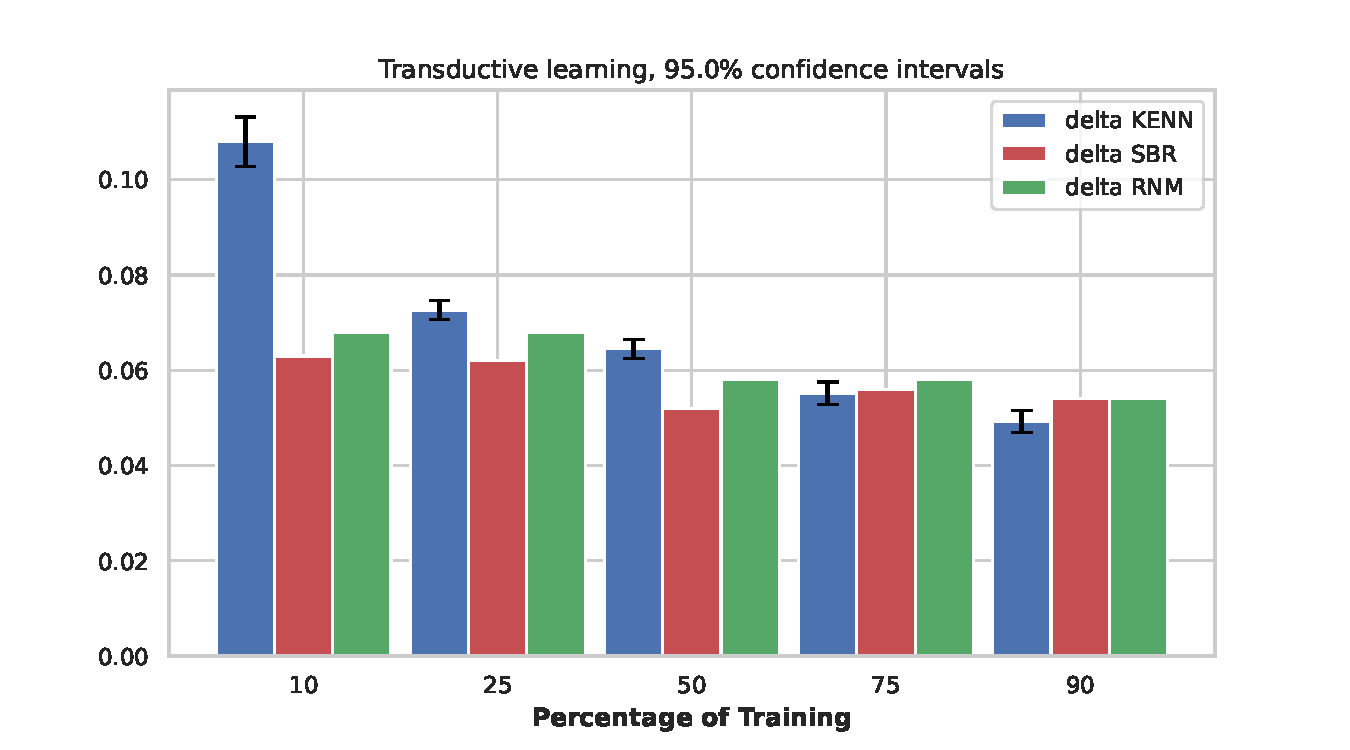
\includegraphics[width=0.8\linewidth]{figures/deltas_transductive.pdf}
		\caption{Relative improvements for the transductive learning task. $95\%$ confidence intervals are provided for our results.}
		\label{fig:transductive_deltas_comparison}
\end{figure}

\begin{figure}
	\centering
	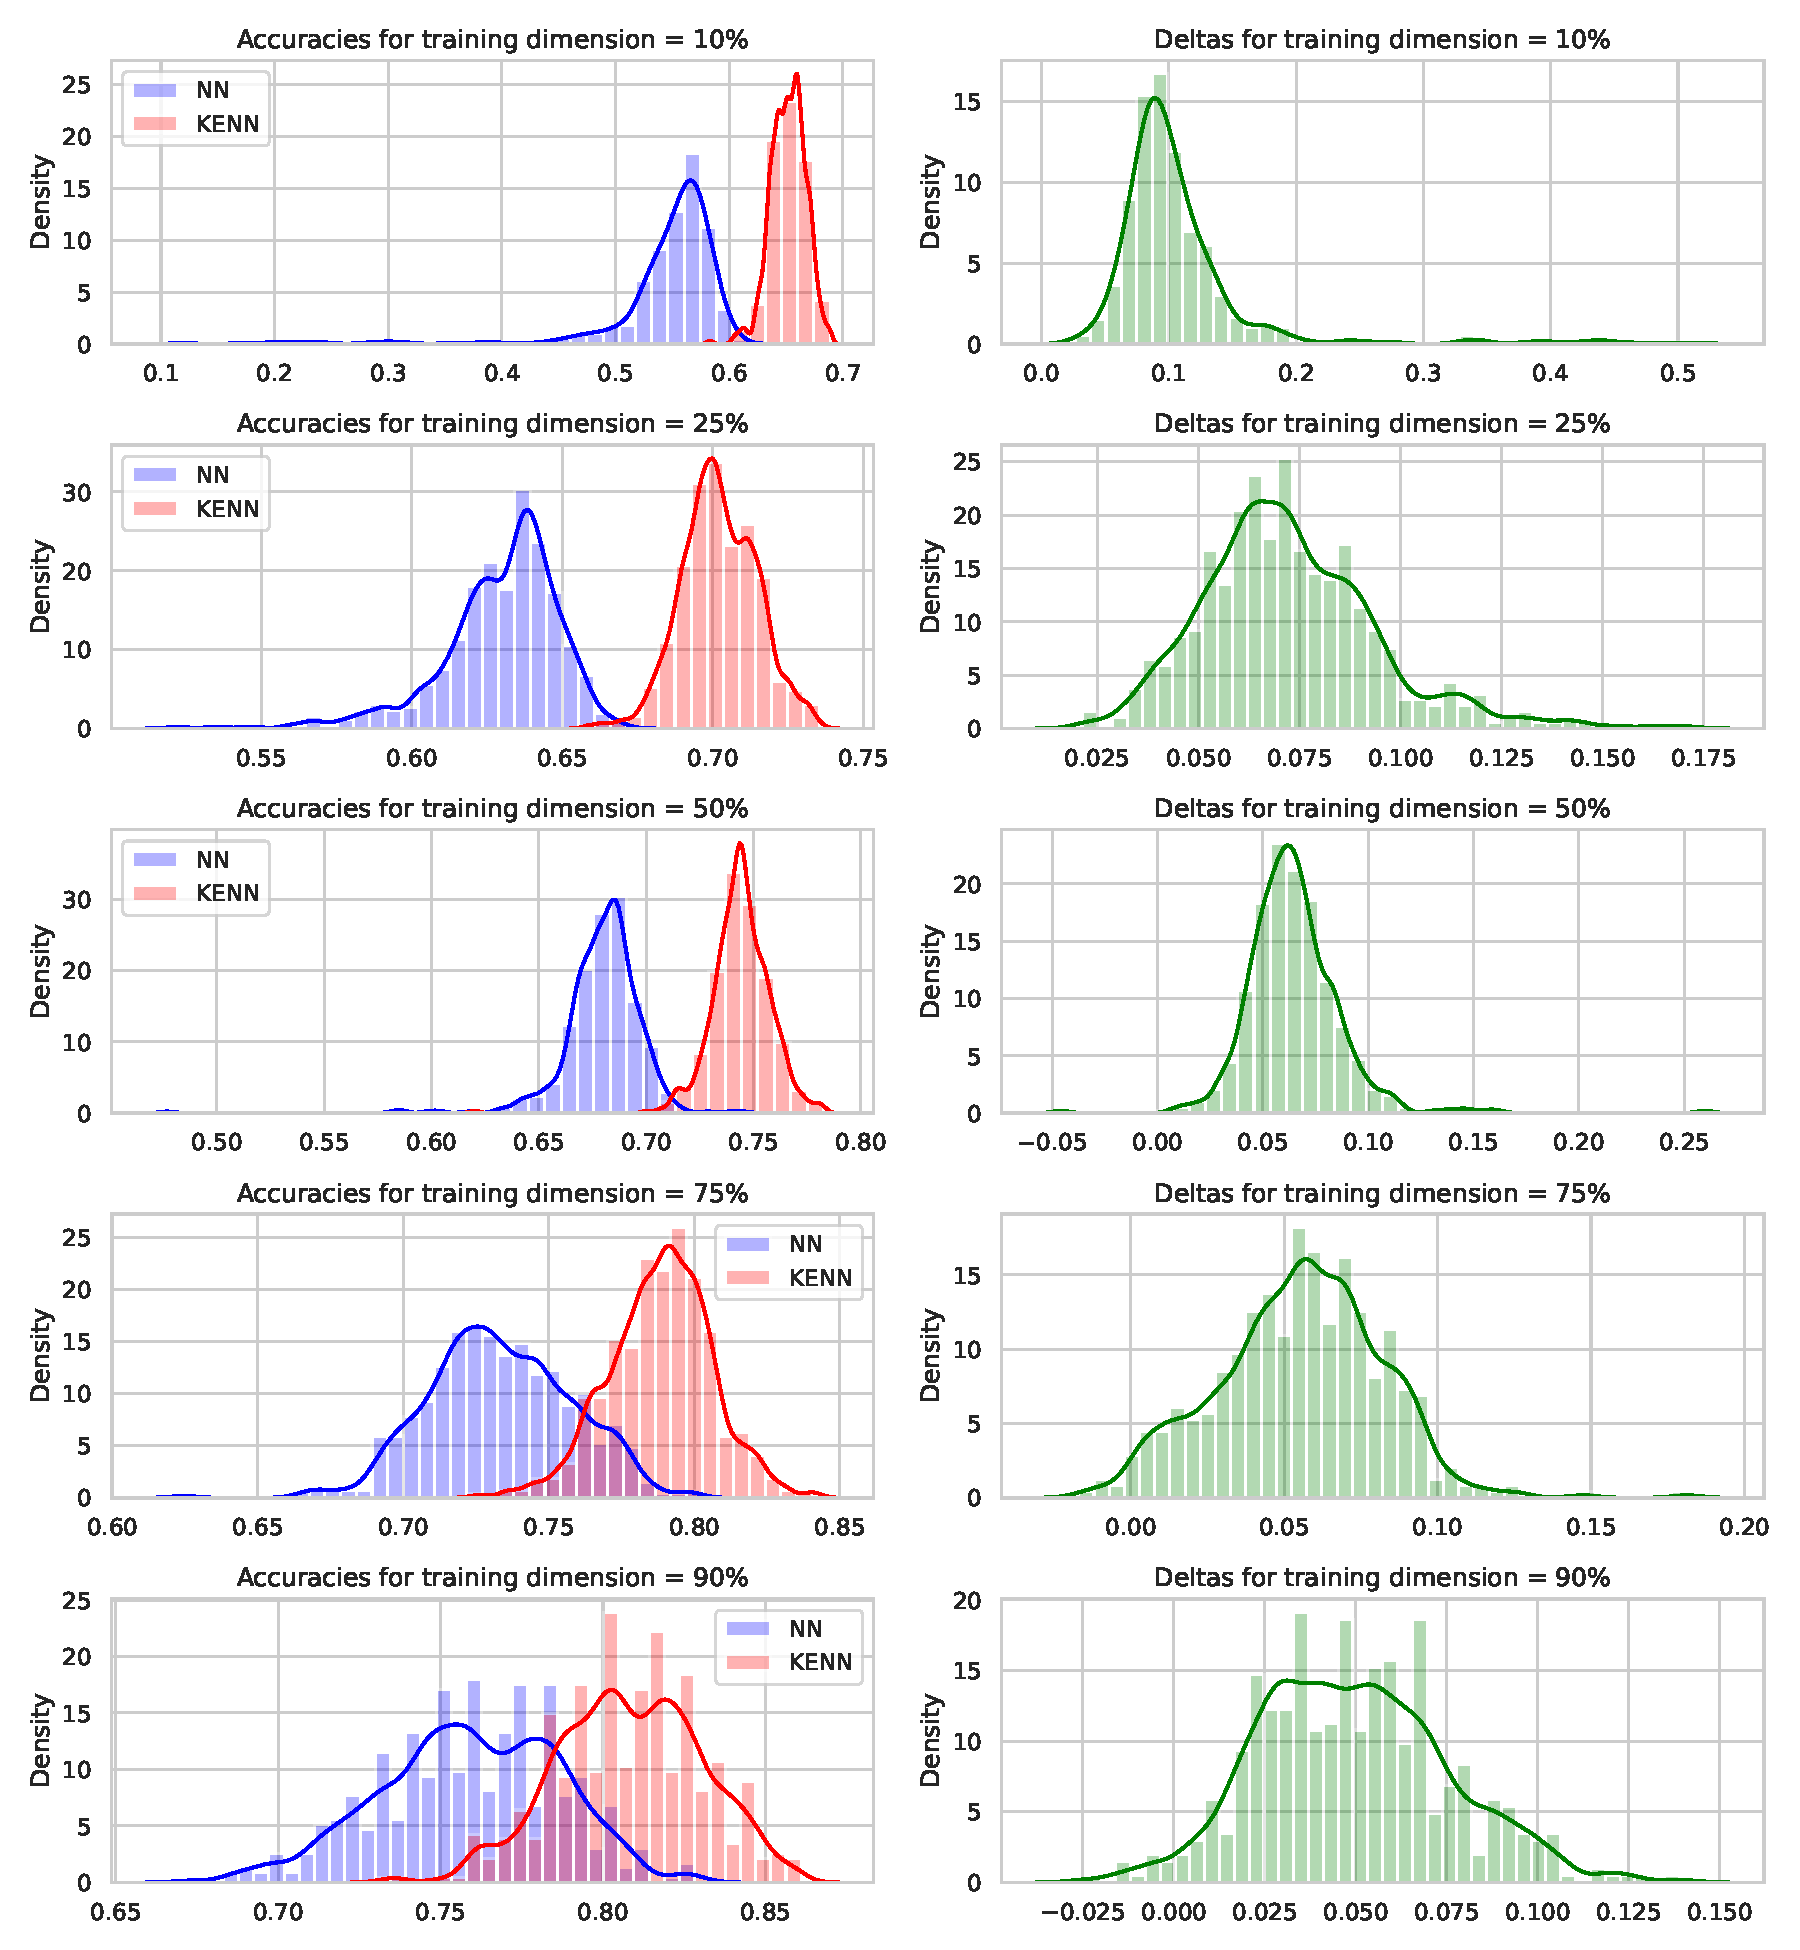
\includegraphics[width=0.95\linewidth]{figures/histograms_transductive.pdf}
	\caption{Histograms showing the distribution of the accuracies for all the different $500$ runs, for the transductive case. On the left, the accuracies of the base NN vs accuracies of KENN. On the right the distribution of the relative improvements.}
	\label{fig:transductive_histograms}
\end{figure}

\begin{table}[h]
	\caption{p-values computed for each learning paradigm and for each training percentage. Values below $10^{-100}$ are reported as $0$.}
	\label{tab:p_vals}
	\centering
	\begin{tabular}{c|cc} 
		\% training & p-value Inductive & p-value Transductive \\
		\hline 
		\rule{0pt}{3ex}    $10$ & $3.22 \cdot 10^{-36}$ & $0$ \\
		$25$ & $0$ & $0$ \\
		$50$ & $0$ & $0$ \\
		$75$ & $2.25 \cdot 10^{-48}$ & $0$ \\
		$90$ & $2.87 \cdot 10^{-9}$ & $0$ \\	
		\hline \hline
	\end{tabular}
\end{table}

\subsection{Clause Weights and satisfaction of the rules}

One of the best features of KENN is its capability to learn the clause weights. This is a fundamental property, since it allows the model to automatically boost the importance of useful rules, and to ignore useless ones. However, to actually verify that KENN is able to correctly learn these weights, we analyzed them after training and investigated on the reasons that lead to their growth or shrinkage.

Specifically, what we care about is to have an empirical evidence that, if a certain clause is particularly important, KENN is able to increase its respective clause weight. We quantify the importance of a specific clause by defining the \textit{clause compliance}, a metric which expresses how much a clause is satisfied on the training data. 

\begin{definition}[Clause Compliance]
	Let $G:=(V,E,T)$ be the current training graph, where $V$ is the set of nodes, $E$ is the set of edges and $T:V\rightarrow \{1,\dots,6\}$ is the function that maps each node to its ground truth class.
	Given one of the output classes $k\in\{1,\dots,6\}$ and the corresponding clause $c_k: \neg k(x) \vee \neg \operatorname{Cite}(x,y) \vee k(y)$, we define the clause compliance of $c_k$ in $G$ as:
	\begin{equation}
	 C(G,c_k) = \frac{\sum_{v \in T_k} \sum_{u \in \mathcal{N}(v)}\mathbf{1}(u\in T_k)}{\sum_{v\in T_k}|\mathcal{N}(v)|}
	\end{equation}
	where $T_k$ is the set of nodes of topic $k$, $\mathcal{N}(v)$ is the number of nodes cited by $v$, and $\mathbf{1}(u\in T_k)$ is equal to $1$ if $u\in T_k$ or $0$ otherwise. In simpler terms, $C(G,c_k)$ is the ratio between the number of citations from papers of topic $k$ to papers of topic $k$ and the total number of citations coming from papers of topic $k$. It is equal to $1$ when always satisfied, and is equal to $0$ when never satisfied. To investigate whether KENN is capable to associate higher weights to clauses with a high clause compliance, we perform $85$ different training runs, and inspect the learned weights for each clause against its clause compliance. We repeat this process for each percentage of the training set. Results are visualized in Figure \ref{fig:corrplots}: by looking at the obtained plots, we can observe that there is a strong correlation between the two variables, which gets more pronounced as the size of the training set increases. Another interesting fact is that, as the clause compliance decreases, an higher variance in the values of the clause weights is observed. For example, looking at the $90\%$ case, we can see that the clause associated to the topic \say{AI} has a mean clause compliance slightly smaller than $0.5$, meaning that this rule is satisfied slightly less than half of the times. By looking at all the values assumed by its clause weight throughout the runs, we can indeed see that the results are very variable with respect to the other topics. This behavior goes against our intuition in some way: if a rule is not useful (like in this case), then the clause weights should monotonically decrease during training, leading to low and tightly packed values for the learned clause weights. In reality, we found that as the compliance of the rules in the data decreases, the learning of their clause weights becomes more randomic: this could be due to a variety of factors, which do not appear to have an obvious or easy explanation. One possible interpretation could be that different randomic initializations of the base NN could lead less compliant clauses to actually produce positive changes, in turn leading KENN to believe that the importance of such a clause should be boosted.
\end{definition}

\begin{figure}
	\centering
	\begin{subfigure}{.5\textwidth}
		\centering
		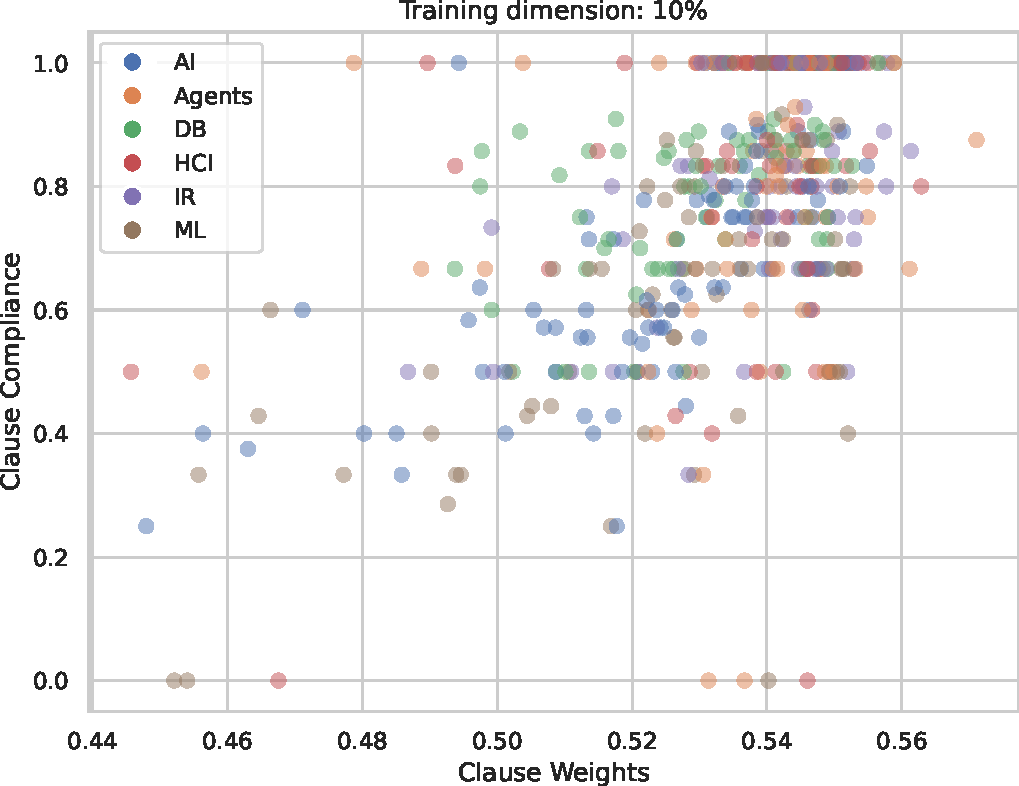
\includegraphics[width=0.95\linewidth]{figures/scatter_10.pdf}
%		\caption{The Clause Enhancer (CE) module.}
		\label{fig:aa}
	\end{subfigure}%
	\begin{subfigure}{.5\textwidth}
		\centering
		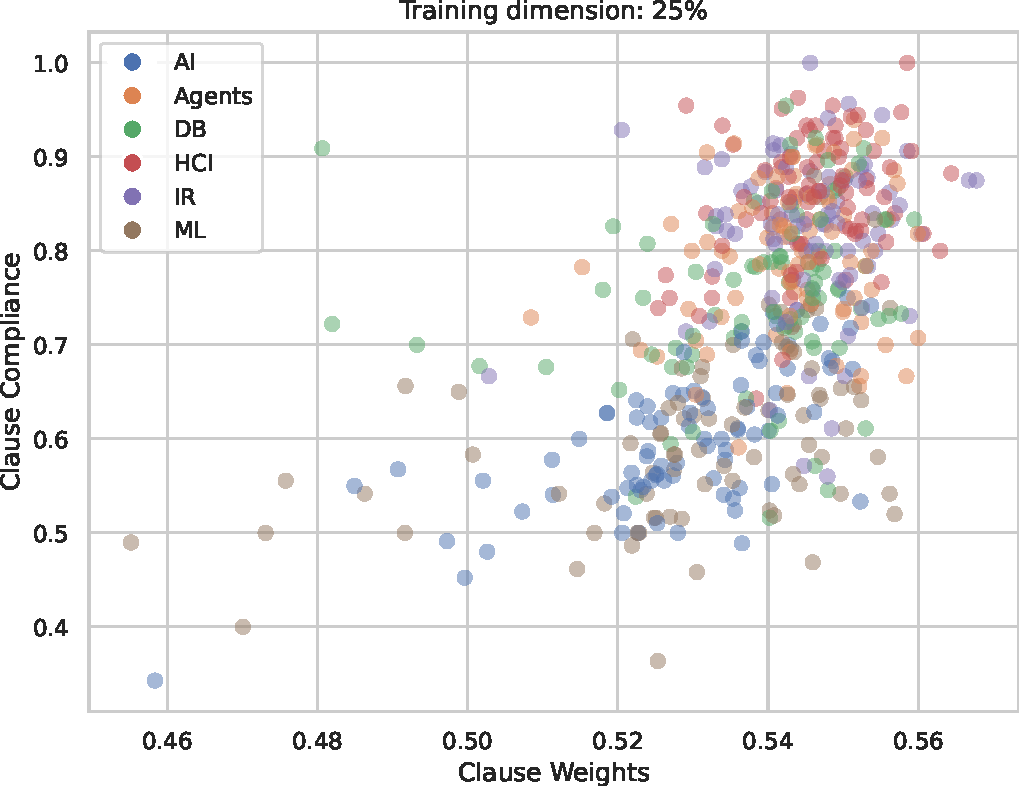
\includegraphics[width=0.95\linewidth]{figures/scatter_25.pdf}
%		\caption{The Knowledge Enhancer (KE) module.}
		\label{fig:vv}	
	\end{subfigure}\\
	\begin{subfigure}{.5\textwidth}
	\centering
	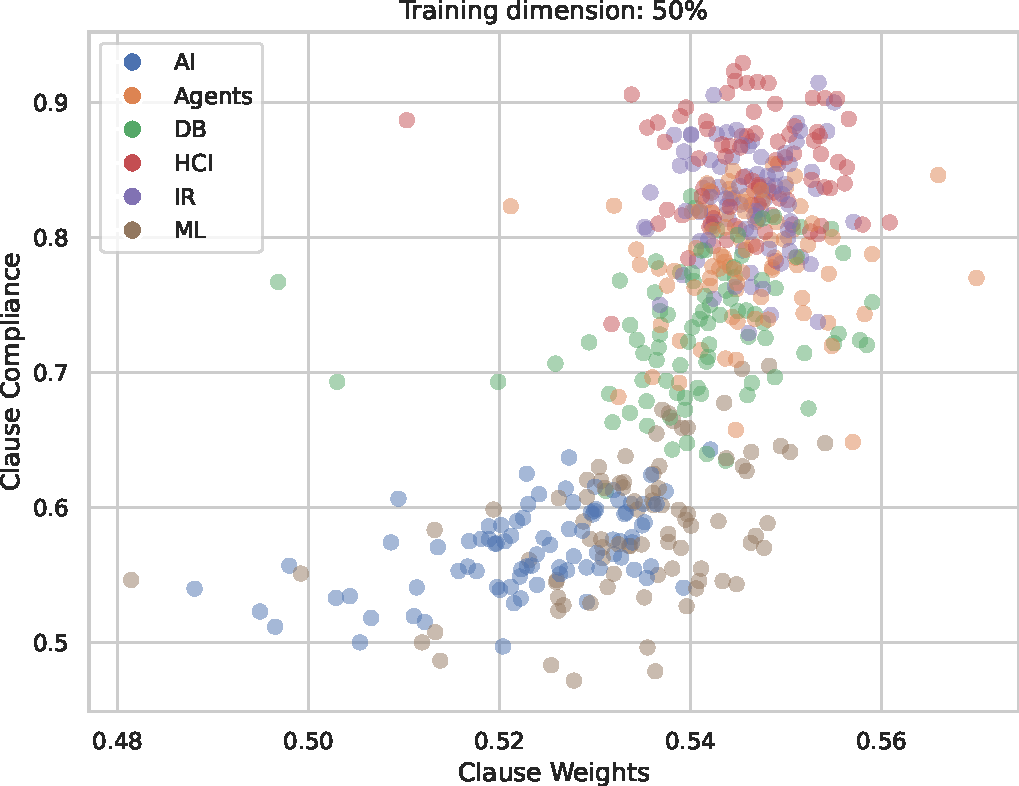
\includegraphics[width=0.95\linewidth]{figures/scatter_50.pdf}
%	\caption{The Clause Enhancer (CE) module.}
	\label{fig:cc}
\end{subfigure}%
\begin{subfigure}{.5\textwidth}
	\centering
	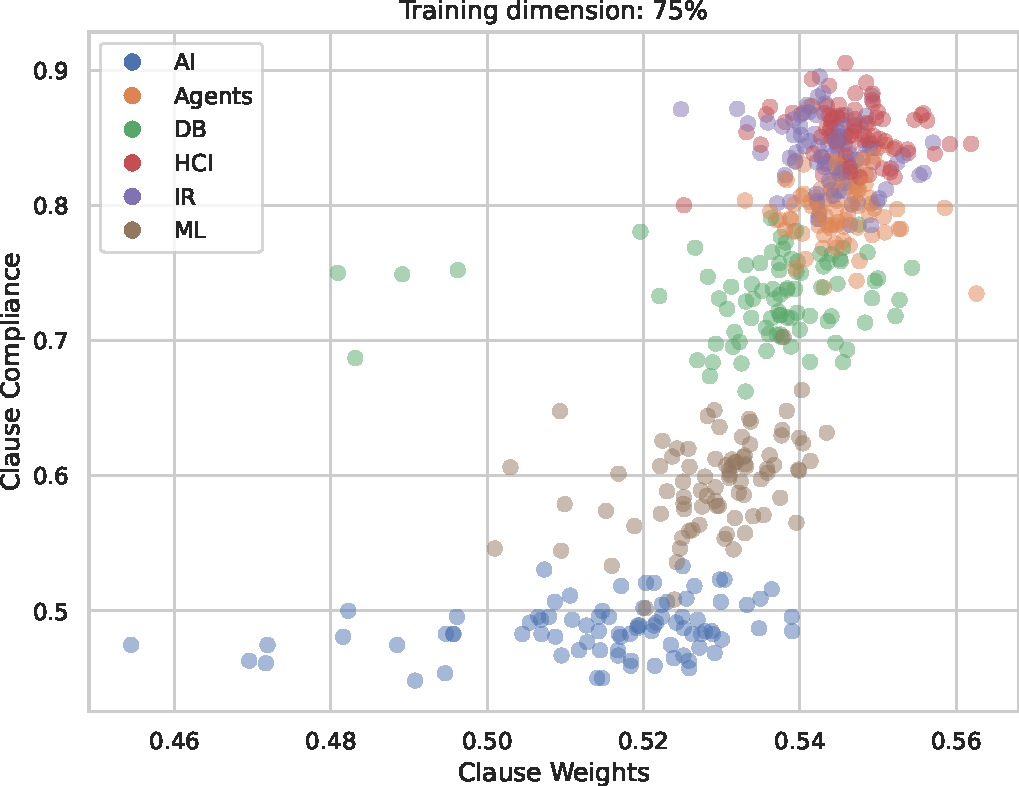
\includegraphics[width=0.95\linewidth]{figures/scatter_75.pdf}
%	\caption{The Knowledge Enhancer (KE) module.}
	\label{fig:dd}	
\end{subfigure}\\
\begin{subfigure}{0.5\textwidth}
	\centering
	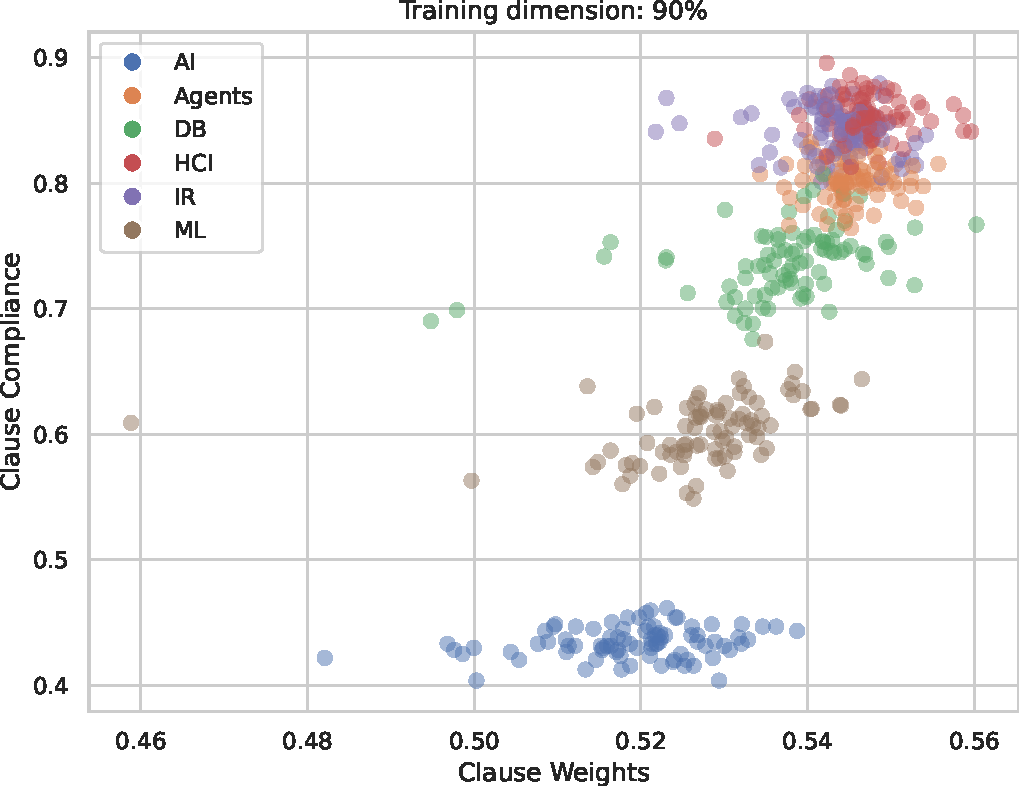
\includegraphics[width=0.95\linewidth]{figures/scatter_90.pdf}
%	\caption{The Knowledge Enhancer (KE) module.}
	\label{fig:ee}	
\end{subfigure}
%	\label{fig:kenn_architecture_unary}
\caption{Scatterplots showing the relation between clause weight and clause compliance, for each clause from $85$ different runs, for each different training percentage. We can observe how, as the training dimension increases, KENN learns to adjust the clause weights according on how much that clause is satisfied in the training set. Each dot in the scatterplots corresponds to a clause in a specific run; the colour of the dot denotes the topic related to that clause.}
\label{fig:corrplots}
\end{figure}

 \section{Explainability in KENN}
 \label{sec:explainability_kenn}
 In this section, we study how to obtain explanations from KENN. In Chapter \ref{chapt:explainability} we studied different kinds of approaches for interpretability and explainability in ML, specifically for the case of NNs. We also analyzed the important distinction between transparent models and post-hoc explainability methods, together with their advantages and disadvantages.
 As we know, KENN can't work on its own: it needs a base NN classifier which has the task of providing the initial predictions. For this reason, KENN can't be considered a completely transparent model just because it is designed to work alongside a standard NN architecture, which is inherently hard to interpret and explain. However, once the initial predictions from the base NN are provided, everything that happens inside the KE can be interpreted; for this reason, KENN can be considered a partially transparent model. Indeed, if we restrict just to the phase where the rules from the knowledge are enforced, everything that happens inside the KE layer is completely transparent. 

 To better justify this claim, let's take into consideration the single components of KENN: the whole layer is composed by the KE, which in turn instantiates several CEs, sums their returned deltas together with the original preactivations, and returns the final, modified predictions. Therefore, the core of the KENN layer is constituted by the CEs. Everything that happens inside a CE is easy to understand to the point that, given the initial preactivations from the base NN and the clause weights, even a human could produce a prediction. These characteristics match the simulatability and decomposbility definitions reported in Section \ref{sec:whatisexplainability}, justifying even more our claim that the KENN can be considered a completely transparent NN layer. In practice, the transparency of the CE module allows us to extract explanations for the predictions given by KENN. To understand how, we propose a simple example. Consider the clause $c : \neg \operatorname{Dog}(x) \vee \operatorname{Animal}(x)$, which expresses the fact that if an object is a dog, then it is also an animal. Now suppose that our model returns the following predictions and deltas:
 $$\operatorname{Dog}(c)=0.7, \operatorname{Animal}(c)=0.2; \quad \delta \operatorname{Dog}(c)=-0.3, \delta \operatorname{Animal}(c)=0.001.$$
 How can we obtain an explanation from the following deltas? To understand this, we first note that:
  $$\neg \operatorname{Dog}(c)=0.3, \operatorname{Animal}(c)=0.2; \quad \delta \neg \operatorname{Dog}(c)=0.3, \delta \operatorname{Animal}(c)=0.001,$$
  where the first two are the truth values for the literals of clause $c$ and the following two are the corresponding deltas, the output of equation (\ref{eq:soft_approx_delta}). By the way the CE works, we know that the value of the highest literal of the clause is the one that will be increased more, since this increases the truth value of clause $c$. For this specific example, the highest literal was $\neg \operatorname{Dog}(c)$, and was increased by $0.3$: this can be explained by the fact that the NN was almost sure that sample $c$ was not an animal, therefore, since we know that $\operatorname{Dog}(c) \Rightarrow \operatorname{Animal}(c)$, then the confidence for $\neg \operatorname{Dog}(c)$ should increase (meaning that the confidence for $\operatorname{Dog}(c)$ should decrease). In even simpler terms, since the NN predicted with high confidence that $c$ is not an animal (note that confidence of $0.2$ for $\operatorname{Animal}(c)$ translates to a confidence of $0.8$ for $\neg \operatorname{Animal}(c)$), then $c$ will not probably be a dog, therefore the truth value of $\operatorname{Dog}(c)$ should decrease. In the end, the final predictions will be $\operatorname{Dog}(c)=0.4, \operatorname{Animal}(c)=0.2001$: note how the base predictions have been corrected by KENN, using the knowledge from the clause $c$. This is just a simple example, but it shows how it is possible, for any prediction and for any clause, to explain the logical reason behind each produced delta, by taking into consideration all the literals of the clause and their relationship. Notice also how these kind of considerations can be converted into the form of natural language explanations, which could be very useful auxiliary tools for researchers and practitioners looking for explanations from the predictions given by KENN.

 Up to now we saw how to extract explanations by inspecting a single clause. However, it is also possible, at inference time, to evaluate the impact on the final predictions of multiple clauses at a time. Specifically, this process can happen at different levels of precision: for example, we might want to study the changes caused by the whole base knowledge, or we might desire to isolate the effects of a small group of clauses. More precisely, given a base knowledge $\mathcal{K}$, and given a subset of clauses $\mathcal{C} \subseteq \mathcal{K}$ for which we want to observe the effects, the delta vector we are looking for is the sum of all the vectors $\delta_c, \forall c \in \mathcal{C}$. However, note that the KE module is designed to compute $\sum_{\mathcal{K}}\delta^c$, while we are interested in $\sum_{\mathcal{C}}\delta^c$: for this reason we will need to intercept the deltas just as they are returned by their respective CEs. Figure \ref{fig:delta_extraction} provides a visualization of this process for the unary and binary case. 
 \begin{figure}
 	\centering
 	\begin{subfigure}{.4\textwidth}
 		\centering
 		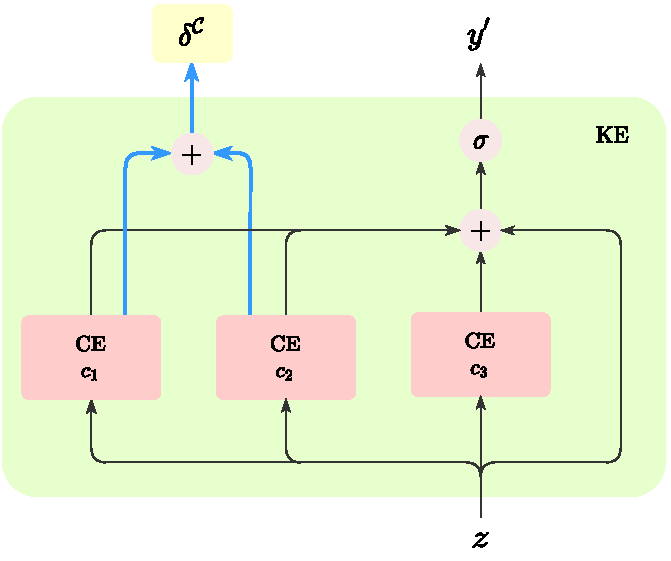
\includegraphics[width=\linewidth]{figures/deltas_extraction_unary.pdf}
 		\caption{Delta extraction from the KE module, for the clauses subset $\mathcal{C}=\{c_1,c_2\}$.}
 		\label{fig:delta_extraction_unary}	
 	\end{subfigure}%
  	\begin{subfigure}{.6\textwidth}
 	\centering
 	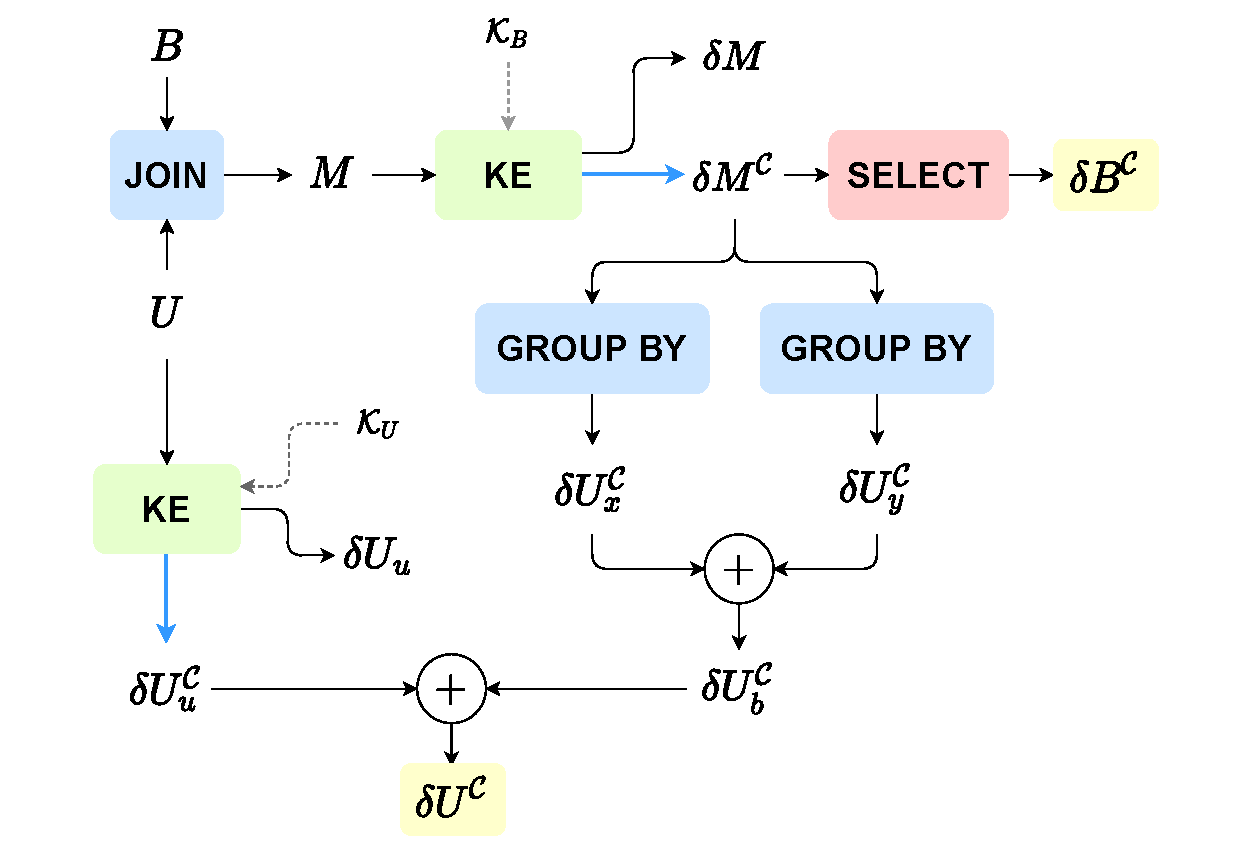
\includegraphics[width=\linewidth]{figures/delta_extractions.pdf}
 	\caption{Delta extraction for the binary case. Note how this process takes place simultaneously with the computation of the whole delta matrices $\delta U$ and $\delta B$ (cf. Figure \ref{fig:kenn_rel_global_scheme}).}
 	\label{fig:delta_extraction_binary}
 \end{subfigure}%
\caption{Process for extracting deltas relative to the clauses in $\mathcal{C \subseteq \mathcal{K}}$. The output deltas are highlighted in yellow for both the unary case (a) and binary case (b). Note that in the binary case the blue arrows are just a shorthand for the extraction process shown on the left.}
\label{fig:delta_extraction}
 \end{figure}
We can also extract the deltas caused by different non overlapping subsets of clauses. Note however that the exact contribution from each different subset can be visualized only when working at the level of preactivations. Indeed, we know that the actual delta at the activation level (denoted in Section \ref{sec:tbf_preac} as $\delta^g$) will change based on the preactivations values, even if the initial delta applied at the preactivation level (denoted in previous section as $\delta^f$) is the same. Recall that we already illustrated this fact in Figure \ref{fig:preacs_deltas_example}. This implies that, when cumulating more deltas from different clauses, we can visualize the exact contribution from each clause at the preactivation level, but we lose this information at the activation level, where the only thing we can observe is the aggregated contribution of all the clauses. A simple example showing this problem is reported in Figure \ref{fig:ex_more_clauses}: 
 \begin{figure}
	\centering
	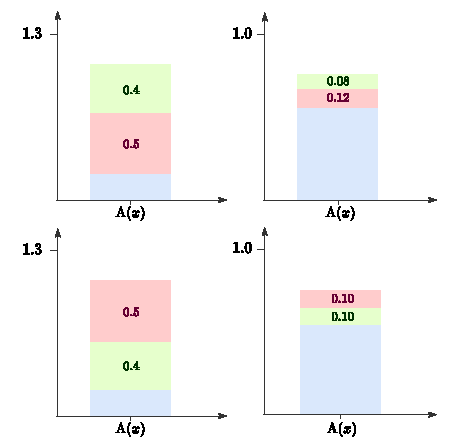
\includegraphics[width=0.5\linewidth]{figures/example_more_clauses.pdf}
	\caption{An example showing the application of two different deltas derived from two different clauses, on a single common literal. On the left, the deltas are applied to the preactivations from the base NN, but in two different orders. Note how, at the activation level,the individual contributions change based on the order of application at the preactivation level,  while the aggregated contribution stays the same.}
	\label{fig:ex_more_clauses}
\end{figure}
here we consider two different clauses $c_1$ and $c_2$, which have the literal $A(x)$ in common, and are identified by different colors (for simplicity, we illustrate only what happens to the common literal $A(x)$). The two clauses produce two deltas: $\delta_{c_1}$ and $\delta_{c_2}$, which are added to the preactivations from the base NN. The figure shows what happens when the deltas are applied in two different orders. First, note that the cumulative effect of $\delta_{c_1}$ and $\delta_{c_2}$, of course, stays the same for both the possible orderings, even at the activation level. This is because:
\begin{equation*}
\sigma(z + \delta_{c_2} + \delta_{c_1}) - \sigma(z) = \sigma(z + \delta_{c_1} + \delta_{c_2}) - \sigma(z).
\end{equation*}
However, note how each individual clause contributes with different quantities, depending on the order of application at the preactivation level. Specifically, if we focus on $c_1$:
\begin{equation*}
\sigma(z + \delta_{c_1}) - \sigma(z) \neq \sigma(z + \delta_{c_1} + \delta_{c_2}) - \sigma(z + \delta_{c_2}).
\end{equation*}
In simple terms, the contribution of each clause at the activation level depends on the order in which the clauses apply their contribution at the preactivation level: the problem is that this order is not defined since all the deltas are applied simultaneously. Therefore, when inspecting the changes caused by more clauses, the only information that we can retain is the aggregated contribution of all of them.

\subsection{Evaluation Metrics}

In real-world problems, one might deal with hundreds or thousands of clauses and/or predicates: the manual inspection of deltas in those cases is not feasible, and in general local explanations are less useful. For this reason, alternative approaches are necessary. For example, one might desire to find a certain score which quantifies how much the contribution from the knowledge (or a subset of the knowledge $\mathcal{C \subseteq \mathcal{K}}$) improved (or worsened) a certain prediction from the base NN.
This score can be defined as follows:
\begin{definition}[Improvement Score]
	Suppose that $x$ is an input sample, to be classified into one or more of $m$ classes. We define the vector of deltas $\hat{\delta^{\mathcal{C}}} = \sigma(z + \delta^{\mathcal{C}}) - \sigma(z)$ where  $\delta^{\mathcal{C}}\in \mathbb{R}^m$ is the delta coming from clauses belonging to $\mathcal{C} \subseteq \mathcal{K}$. Given vector of ground truth labels $l \in \{-1,1\}^m$, where the $i$-th entry is equal to $1$ if $x$ belongs to the $i$-th class, and $-1$ otherwise, then the improvement score for $x$ with respect to $\mathcal{C}$ is defined as follows:
	\begin{equation}
	\label{eq:impr_score}
	IS(x,\mathcal{C})=\sum_{i=1}^m \hat{\delta^{\mathcal{C}}}_i \cdot  l_i =  \hat{\delta^{\mathcal{C}}}^{\top} \cdot  l.
	\end{equation}
	The improvement score quantifies the positive contribution of the KENN layer for the current prediction.
\end{definition}
Note that $\hat{\delta^{\mathcal{C}}}$ is simply the vector of deltas at the activation level. In simple terms, what happens in equation (\ref{eq:impr_score}) is that each term of the delta vector will produce a positive contribution only when its sign is the same as the corresponding ground truth label. This is because we want KENN to increase the confidence for positive classes, and decrease it for negative classes. This score can be useful for several applications: for example, we might want to analyze the predictions for which KENN gave the most improvements or, vice-versa, we might want to see where KENN has actually provided worse results with respect to the base NN. To do that we can simply order the predictions based on this score: an increasing order will give in the first places the most problematic predictions, where KENN gave the worst results. On the contrary, a decreasing score will provide first the best results.


Now, recall that KENN aggregates the deltas of all the clauses by simply summing the individual deltas: this is very convenient since it makes KENN fast and scalable. However, we saw that this kind of aggregation may be too simplistic, and may cause inconsistencies in the case where multiple clauses disagree on how certain truth values should be changed. In order to diagnose this kind of behavior on a trained KENN model, we can define another score:

\begin{definition}[Disagreement Score]
	Using the previously defined notation, we can define the disagreement vector for sample $x$ with respect to the subset of clauses $\mathcal{C}$ as follows:
	\begin{equation}
DV(x, \mathcal{C}) = \sum_{c\in\mathcal{C}}\left|\hat{\delta_c}\right| - \left|\sum_{c\in\mathcal{C}}\hat{\delta_c} \right|.
	\end{equation}
Given $DV(x, \mathcal{C})$, we can define two different scores:
\begin{itemize}
	\item $DS(x,i,\mathcal{C}) = DV(x, \mathcal{C})_i$: the disagreement score for sample $x$, with respect to the $i$-th predicate;
	\item $DS(x,\mathcal{C}) = \sum_i DV(x, \mathcal{C})_i$: the cumulated disagreement score for sample $x$ with respect to all the predicates. 
\end{itemize}
This score quantifies the amount of inconsistencies and disagreement among the clauses belonging to $\mathcal{C}$: a score of $0$ implies perfect agreement between all the clauses, while an higher score reflects an higher disagreement. We recall that two clauses are said to disagree if, given a common literal, the deltas that they produce for that literal have different signs. Not also how we can choose to restrict the analysis to a single predicate (or a subset of predicates), or to consider them all together.
\end{definition}
%An interesting property of these defined scores is that we can also focus on specific predicates: specifically, for each sample $x$, we can compute the improvement or disagreement score for a certain subset of predicates by simply retaining their relative deltas. 

Also in this case, one could rank the predictions with respect to the disagreement score, to evaluate which clauses disagree more; we can also choose to measure the disagreement on specific predicates, or on all of them. This can be useful in different situations, like during debugging or for the knowledge selection phase.

To conclude, we saw that, in general, explanations extracted from KENN can be useful mostly to evaluate the impact of the knowledge, and can allow the user to refine it, by adding or removing rules that proved to be useful or damaging. We also saw that, when inspecting single clauses, more expressive explanations can be extracted: specifically, thanks to the transparency of the CE, simple and human readable explanations can be derived and even converted in natural language form. We remark, however, that this transparency is just partial and limited to the knowledge enforcement stage: indeed, the base NN remains an opaque component of the whole model, even if used in conjunction with KENN.
 


